% !TeX encoding   = UTF-8
\documentclass[msc]{ppgccufmg} % ou [msc] para dissertações
                                        % de mestrado. Para propostas ou
                                        % projetos, usar [phd,project],
                                        % [msc,proposal], etc.
\usepackage[brazil]{babel} % ajusta vários detalhes para
                           % documentos escritos em português,
                           % principalmente hifenização
\usepackage[T1]{fontenc}   % permite a hifenização de
                           % palavras acentuadas
\usepackage[utf8x]{inputenc} % ou [utf8x] para quem prefere
                             % usar a codificação UTF-8
\usepackage{graphicx} % define o comando \includegraphics
                      % para a inclusão de Figuras
%\usepackage[square]{natbib} % permite citações naturalmente
                            % integradas ao texto
\usepackage[a4paper,
portuguese,
bookmarks=true,
bookmarksnumbered=true,
linktocpage,
colorlinks=true,
citecolor=black,
urlcolor=black,
linkcolor=black,
filecolor=black,
]{hyperref}
\usepackage[table,xcdraw]{xcolor}
\usepackage{amsmath}
\usepackage{multirow}
%\usepackage{todonotes}
\usepackage[colorinlistoftodos,prependcaption,textsize=tiny]{todonotes}
\usepackage{pdfpages}
\usepackage{capt-of}
\usepackage{svg}
\usepackage{epsf}
\usepackage{epstopdf}
\usepackage{lscape}
\usepackage{graphicx}
\usepackage{booktabs}
\hyphenation{pos-ta-gem ou-tros pro-ble-ma a-na-li-sar des-co-brir su-ge-rir
            e-qui-vo-ca-das re-la-ti-vos es-pe-ra-mos fun-ci-o-na-li-da-des
            hi-e-rar-qui-as es-ta-be-le-ci-men-to te-nham res-trin-gir
            o-fe-re-ci-das re-qui-si-to tra-ba-lhos do-cu-men-ta-\c{c}\~ao
            re-gis-trar ges-to-res al-te-ra-\c{c}\~o-es di-fe-ren-tes
            o-pe-ra-\c{c}\~ao re-cu-pe-ra-\c{c}\~ao pre-ver de-di-can-do
            ge-ne-ra-li-za-\c{c}\~ao tra-ba-lham res-pos-tas hi-e-rar-qui-a
            re-a-li-za-do au-to-ma-ti-za-das ca-te-go-ri-za-\c{c}\~ao
            co-nhe-ci-men-to tra-ba-lhos me-lho-ri-as re-gis-tros
            Re-cu-pe-ra\c{c}\~ao pon-tu-a-\c{c}\~ao res-pos-tas}
\begin{document}

\ppgccufmg{title={Um Estudo de Ferramentas de \\
Gerenciamento de Requisição de Mudança},
author={Vagner Clementino},
authorrev={Clementino, Vagner},
university={Universidade Federal de Minas Gerais},
course={Ciência da Computação},
address={Belo Horizonte},
date={2017-05-31},
advisor={Rodolfo F. Resende},
keywords={Manutenção de Software, Ferramentas, Extensões},
%approval={img/approvalsheet.eps},
%approval=[-2.5cm][1]{aprovalsheet},
abstract={Resumo}{./resumo/resumo},
% abstract=[english]{Abstract}{./abstract/abstract},
%abstract={Resumo Estendido}{./resumoest/resumoest},
%dedication={./dedicatoria/dedicatoria},
%ack={./agradecimentos/agradecimentos},
	epigraphtext={O antigo, inimigo cedeu o espaço\\
Pra um desafio ainda maior\\
Se manter de pé,\\
Contra o que vier,\\
Vencer os medos,\\
Mostrar ao que veio,\\
Ter o foco ali,\\
E sempre seguir\\
Rumo a vitória!}{Vitória \@-\@ Dead Fish},
indexkeys={1.~Computação --- Teses. 2.~Engenharia de Software --- Teses.
    I.~Orientador. II.~Título.},
}
%\newpage
%\listoftodos[Notes]
%Novos comanddos
\newcommand{\todobegin}[1]{\todo[inline]{\#BEGIN\@: #1}}
\newcommand{\todoend}{\todo[inline]{\#END}}

\newcommand{\sugestao}[2]{\fbox{
		\begin{minipage}{.9\textwidth}
			\textbf{Sugestão \##1:} #2
		\end{minipage}
	}
}

%Incluindo o fonte do Capítulo 01
%%%%%%%%%%%%%%%%%%%%%%%%%%%%%%%%%%%%%%%%%%%%%%%%%%%%%%%%%%%%%%%%%%%%%%%%%%%%%%%%%%%%%%%%%%%%%%%%%%%%%%%%%%%%
%Objetivo: Introduzir os conceitos envolvidos na dissertação bem como do trabalho realizado.
%		   A ideia é que qualquer pessoa que leia a introdução consiga ter uma visão geral
%		   sobre a dissertação.
%Autor: Vagner Clementino <vagnercs@dcc.ufmg.br> e Rodolfo Resende <rodolfo@dcc.ufmg.br>
%Data Criação: Dom Set 18 22:55:43 BRT 2016
%Data Modificação: Dom Set 18 22:55:57 BRT 2016
%Data Revisão: Dom Set 18 22:56:08 BRT 2016
%%%%%%%%%%%%%%%%%%%%%%%%%%%%%%%%%%%%%%%%%%%%%%%%%%%%%%%%%%%%%%%%%%%%%%%%%%%%%%%%%%%%%%%%%%%%%%%%%%%%%%%%%%%%
\chapter{Introdução}
\label{ch:intro}
\todo[inline]{O objetivo de seção é introduzir ao leitor na disciplina de Engenharia de Software, em
especial quanto aos tipos de manutenção descritos na literatura e a utilização de uma ferramenta
para o seu gerenciamento}

Dentro do ciclo de vida de um produto de software o processo de manutenção tem
papel fundamental. Devido ao seu alto custo, em alguns casos chegando a 60\%
do preço final~\cite{kaur2015review}, as atividades relacionadas a manter e evoluir software tem sua
importância considerada tanto pela comunidade científica quanto pela indústria.

Desde o final da década de 1970~\cite{Zelkowitz:1979:PSE:578504} percebe-se o aumento do custo
referente as atividades de  manutenção de software. Nas décadas de 1980 e 1990 alguns trabalhos
tiveram seu foco no desenvolvimento de modelos de mensuração do custo para manter o
software~\cite{Herrin:1985:SMC:323287.323383,hirota1994approach}. Apesar da evolução das metologias
de manutenção a estimativa é que nas últimas duas décadas o custo de manutenção tenha aumentado em
50\%~\cite{koskinen2010software}. Esta tendência pode ser observada na
Figura~\ref{fig:software-maintence-costs} no qual é possível verificar a evolução do custo da
manutenção de software como fração do custo total do produto.

\begin{figure}
\centering
\includegraphics[width=0.7\linewidth]{./chapter-intro/img/software-maintence-costs}
\caption{Evolução da manutenção de software como percentual do custo total.	Extraído de~\cite{engelbertink2010save}}
\label{fig:software-maintence-costs}
\end{figure}

Uma vez que o software entra em operação, anomalias são descobertas, mudanças ocorrem no ambiente
de operação e novos requisitos são solicitados pelo usuário. Todas estas demandas devem ser
solucionadas na fase de Manutenção que inicia efetivamente com entrega do sistema, contudo, certas
atividades ocorrem antes.

A \textit{Manutenção}, dentre outros aspectos, corresponde ao processo de modificar um componente ou
sistema de software após a sua entrega com o objetivo de \textit{corrigir falhas, melhorar o
	desempenho ou adaptá-lo devido à mudanças ambientais}~\cite{{159342}}. 
De maneira relacionada, \textit{Manutenibilidade} é a propriedade de um sistema ou componente de software em relação ao grau
de \textit{facilidade} que ele pode ser corrigido, melhorado ou adaptado~\cite{{159342}}.

Verificamos na literatura certa discussão sobre a diferença entre manutenção e evolução de software.
Percebe-se ainda que pesquisadores e profissionais utilizam evolução como substituto preferido para
manutenção~\cite{Bennett:2000:SME:336512.336534}. Todavia, não está no escopo desta dissertação
discutir e apresentar as diferenças entre os conceitos. Neste sentido, utilizamos os termos \textit{manter} e
\textit{evoluir} software de forma intercambiáveis.

As manutenções em software podem ser divididas em \textit{Corretiva, Adaptativa, Perfectiva e
	Preventiva}~\cite{Lientz:1980:SMM:601062,159342}. A ISO 14764 discute
os quatro tipos de manutenções, conforme já descrito, e além disso propõe que exista um elemento comum
denominado \textit{Requisição de Mudança} que representa as características comuns a todas aqueles
tipos de manutenção.

Por conta do volume das Requisições de Mudança se faz necessária a utilização de
ferramentas com o objetivo de gerenciá-las. Esse controle é geralmente
realizado por \textit{Ferramentas de Gerenciamento de Requisição de Mudança -~FGRM}, que auxiliam os
desenvolvedores na correção de forma individual ou colaborativa de defeitos (bugs), no
desenvolvimento de novas funcionalidades, dentre outras tarefas relativas à manutenção de software.
A literatura não define uma nomenclatura comum para este tipo de ferramenta. Em alguns estudos é
possível verificar nomes tais como Sistema de Controle de Defeito -~Bug Tracking Systems, Sistema de
Gerenciamento da Requisição -~Request Management System, Sistemas de Controle de Demandas (SCD)-
Issue Tracking Systems. Todavia, de modo geral, o termo se refere as
ferramentas utilizadas pelas organizações para \textit{gerir as Requisições de Mudança}. Estas
ferramentas podem ainda ser utilizadas por gestores, analistas de qualidade e usuários finais para
atividades tais como gerenciamento de projetos, comunicação, discussão e revisões de código. Neste
trabalho utilizaremos o termo \texttt{Ferramentas de Gerenciamento de Requisições de Mudança} (FGRM)
ao referimos a este tipo de ferramenta.  A Tabela~\ref{tab:exemplo} apresenta alguns exemplos de
software que podem ser classificadas como FGRM's. Também são listados serviços da Internet que
oferecem funcionalidades presentes nas FGRM na forma de Software como
Serviço~\cite{fox2013engineering}.

\begin{table}[ht]
	\centering
	\resizebox{\textwidth}{!}{%
		\begin{tabular}{llll}
			\hline
			\multicolumn{2}{c}{\textbf{Ferramentas}}           & \multicolumn{2}{c}{\textbf{Serviços da Internet}} \\ \hline
			Bugzilla & https://www.bugzilla.org/               & SourceForge    & https://sourceforge.net/    \\ \hline
			MantisBT & https://www.mantisbt.org/               & Lauchpad       & https://launchpad.net/      \\ \hline
			Trac     & https://trac.edgewall.org/              & Code Plex      & https://www.codeplex.com/   \\ \hline
			Redmine  & www.redmine.org/                        & Google Code    & https://code.google.com/    \\ \hline
			Jira     & https://www.atlassian.com/software/jira & GitHub         & https://github.com/         \\ \hline
		\end{tabular}%
	}
	\caption{Exemplos de ferramentas e serviços da Internet. Adaptado de~\cite{cavalcanti2014challenges}}\label{tab:exemplo}
\end{table}

\section{Motivação}
\label{sec:intro-motivacao}


\todo[inline]{O objetivo desta seção é apresentar a motivação do estudo. Em síntese, tenta responder
a seguinte pergunta: Por que dentro do contexto da manutenção de software estudar as Ferramentas de
Gerenciamento de Requisição de Mudança é IMPORTANTE?}

Diante da maior presença de software em todos os setores da sociedade
existe um interesse por parte da academia e da industria no desenvolvimento de
processos, técnicas e \textit{ferramentas} que reduzam o esforço e o custo das tarefas
de desenvolvimento e manutenção de software. Neste linha, o trabalho de Yong \&
Mookerjee~\cite{1423995}  propõe um modelo que reduz os custos de manutenção e reposição durante a
vida útil de um sistema de software. O modelo demonstrou que em algumas situações é \textit{melhor
	substituir um sistema do que mantê-lo}. Este problema é agravado tendo em vista que o custo de
manutenção que alguns necessita que 60\% dos desenvolvedores dedicados à tarefas de manutenção de sistemas~\cite{Zhang_2003}.

Diversos projetos de software, especialmente durante as etapas de desenvolvimento e teste do
software, necessitam de uma ferramenta para gerenciar as suas Requisições de Mudança tendo em vista
o seu volume bem como pela grande quantidade de pessoas inserir dados sobre os erros
encontrados~\cite{1407819}, por exemplo. Este tipo de ferramenta vêm sendo utilizados em projetos de
código aberto (Apache, Linux, Open Office) bem como em organizações públicas e privadas
(NASA,IBM).

Não obstante, alguns estudos demonstram que as FGRM's desempenham um papel além daquele de gerenciar
os pedidos de manutenção e evolução do software. Avaliando o controle de demandas como um processo
social, Bertram et al.~\cite{Bertram:2010:CCB:1718918.1718972} realizaram um estudo qualitativo em
FGRM's quando utilizados por pequenas equipes de desenvolvimento de software. Os resultados
mostraram que este tipo ferramenta não é apenas um banco de dados de rastreamento de defeitos,
recursos ou pedidos de informação, mas também atua como um ponto focal para a comunicação e
coordenação para diversas partes interessadas (stakeholders) dentro e fora da equipe de software. Os
clientes, gerentes de projeto, o pessoal envolvido com a garantia da qualidade e programadores,
contribuem em conjunto para o conhecimento compartilhado dentro do contexto das FGRM's.
 
No trabalho de Breu et al.\cite{Breu:2010:INB:1718918.1718973} o foco é analisar o papel dos FGRM's
no suporte à colaboração entre desenvolvedores e usuários de um software. A partir da análise
quantitativa e qualitativa de defeitos registrados em uma FGRM de dois projetos de software livre
foi possível verificar que o uso da ferramenta propiciou que os usuários desempenhassem um papel
além de simplesmente reportar uma falha: a participação ativa e permanente dos usuários finais foi
importante no progresso da resolução das falhas que eles descreveram.


Um outro importante benefício da utilização das FGRM é que as mudanças no software podem ser
rapidamente identificada e reportada para os desenvolvedores~\cite{anvik2005coping}. Além disso, eles podem ajudar a estimar
o custo do software, na análise de impacto, planejamento, rastreabilidade, descoberta do
conhecimento~\cite{cavalcanti2013bug}.

Não obstante, no contexto de utilização desta ferramentas diversos desafios se apresentam:
duplicação RM's, pedidos de modificação que são abertos inadvertidamente, grande quantidade de RM's
que devem ser atribuídas as desenvolvedores, bugs descrito de forma incompleta, análise de
impacto das RM's e RM's atribuídas de maneira incorreta~\cite{cavalcanti2014challenges}.  Diante de
tantos problemas e desafios é importante entender como aquele tipo de ferramente vêm sendo utilizada
bem como analisar o que está sendo proposta na literatura com objetivo de melhor as funcionalidades
oferecidas pelas FGRM.
%
%No trabalho de Junio et al.~\cite{5741246} é proposto um processo denominado
%PASM (Process for Arranging Software Maintenance Requests) que propõe lidar com
%tarefas de manutenção como projetos de software. Para tanto, utilizou-se
%técnicas de análise de agrupamento (clustering) a fim de melhor compreender e
%comparar as demandas de manutenção. Os resultados demostraram que depois de
%adotar o PASM os desenvolvedores tem dedicado um tempo maior para análise e
%validação. De outra forma, relacionada um menor tempo foi dedicado às tarefas
%de execução e codificação.
%
%No estudo realizado por Bettenburg et al.~\cite{bettenburg2008makes} foi
%desenvolvida uma pesquisa (\textit{survey}) entre desenvolvedores e usuários
%dos projetos Apache\footnote{\url{http://www.apache.org/}},
%Eclipse\footnote{\url{https://www.eclipse.org}} e
%Mozilla\footnote{\url{https://www.mozilla.org}} a fim de verificar o que
%produziria uma boa FGRM\@. Os resultados demonstraram que do ponto de vista dos
%desenvolvedores eram consideradas úteis funcionalidades tais como reprodução do
%erro, rastros de pilhas (stack traces) e casos de testes. A partir deste
%resultado foi construído um protótipo capaz de conduzir os usuários na coleta e
%fornecimento de um maior número de informações úteis para a resolução do
%defeito reportado.
%
%
%Em Zimmermann et al.~\cite{5070993} é discutido a importância de que a
%informação descrita em uma Requisição de Mudança seja relevante e completa a
%fim de que o defeito reportado seja resolvido rapidamente. Contudo, na prática,
%a informação apenas chega ao desenvolvedor com a qualidade requerida após
%diversas interações com o usuário afetado. Com o objetivo de minimizar este
%problema os autores propõe um conjunto de diretrizes para a construção de um
%ferramenta capaz de reunir informações relevantes a partir do usuário e
%identificar arquivos que precisam ser corrigidos para resolver o defeito.
%

%No trabalho de Kononenko et al.~\cite{Kononenko:2014:DED:2591062.2591075} é
%apresentada uma ferramenta denominada \textit{DASH} cujo objetivo é agrupar as
%demandas que são relevantes para as atividades de um desenvolvedor.
%Naturalmente todas as demandas ditas relevantes deveriam estar sob a
%responsabilidade de um mesmo programador. O principal objetivo desta ferramenta
%é aumentar a Consciência Situacional (Situational Awareness) dos
%desenvolvedores. Segundo os autores, o principal ganho do uso da ferramenta é
%que os programadores podem gerenciar melhor o excesso de informação e ficar
%mais ciente da evolução das demais demandas do sistema.
%
%Na ferramenta proposta por Thung et al.~\cite{Thung:2014:DIT:2642937.2648627} o
%foco é na determinação de defeitos duplicados. A contribuição deste trabalho é
%a integração do estado da arte de técnicas não supervisionadas para detecção de
%falhas duplicadas conforme proposto por Runeson et
%al.~\cite{Runeson:2007:DDD:1248820.1248882}. A ferramenta utiliza o Modelo de
%Vetor Espacial (Vetor Space Model) como métrica de similaridade entre os
%defeitos e fornece aos desenvolvedores uma lista de possíveis duplicatas.


%A manutenção não necessariamente exige que o processo de software envolvido
%seja o tradicional. Percebe-se alguns exemplos de adoção das práticas ágeis
%para fins de manutenção e evolução do software~\cite{kajko2009model, Heeager2015, Devulapally2015,Naz2016}. Tal
%tendência não é surpreendente tendo em vista que os métodos ``ágeis'' enfatizam
%características úteis à eficiência da implementação de software, tais como desenvolvimento incremental e teste contínuo que agregam valor para a evolução e manutenção eficaz de um sistema
%\cite{thomas2006agile}. Dentro desta tendência verifica-se a necessidade de que as ferramentas envolvidas no suporte à manutenção de software se adéquem à este nova forma de manter software. 
%


\section{Análise do Problema}
\label{sec:intro-problema}

\todo[inline]{OBJETIVO: Apresentar o problema que esta dissertação pretende resolver. O problema
	deverá ser definido claramente ou deverão ser apresentadas provas da importância do mesmo dentro
do escopo da Engenharia de Software}

O desenvolvimento e a manutenção de software envolvem diversos tipos de métodos, técnicas e
ferramentas. Em especial no processo de manutenção, um importante aspecto são as diversas
Requisições de Mudanças que devem ser gerenciadas. Este controle é realizado pelas FGRM's cujo o uso
vem crescendo em importância, sobretudo, por sua utilização por gestores, analistas da qualidade e
usuários finais para atividades como tomada de decisão e comunicação. How-
ever, most bug tracking systems are far from perfect. Many
of them are merely better interfaces to a database that stores
all reported bugs

Many
of them are merely better interfaces to a database that stores
all reported bugs. As a result, they often ask too much from
end-users who are not familiar with development practices.
At the same time they cause frustration for developers who
are disappointed about the quality of bug reports submitted
by users.

Apesar da inegável importância das FGRM's, percebe-se um aparente desacoplamento deste tipo de
ferramenta com as necessidades das diversas partes interessadas (stakeholders) na manutenção e
evolução de software. A utilização de  \textit{``demanda''} como conceito central para Ferramentas de Gerenciamento de
Requisição de Mudanças (FGRM) parece ser distante das necessidades práticas dos projetos de
software, especialmente no ponto de vista dos desenvolvedores
\cite{Baysal:2013:SAP:2486788.2486957}.

Um exemplo deste desacoplamento deste tipo de ferramenta com a necessidade de seus usuários pode ser visto no
trabalho proposto por Baysal \& Holme \cite{baysal2012qualitative} no qual desenvolvedores que
utilizam o Bugzilla\footnote{\url{https://www.bugzilla.org}} relatam a dificuldade em manter uma
compreensão global das RM's em que eles estão envolvidos. Segundo os desenvolvedores seria
interessante que a ferramenta tivesse um suporte melhorado para a Consciência Situacional
-~Situational Awareness. Em síntese, eles gostariam de estar cientes da situação global do projeto
bem como das atividades que outras pessoas estão realizando.

Com o objetivo de melhorar as FGRM (issue tracking system), mediante a melhoria daquilo que é
reportado aos dessenvolvedores, Zimmermann e outros discute quatro dimensões de melhorias deste tipo
de ferramenta, conforme esquematizado na Figura~\ref{fig:dimensoes_melhorias_fgrm}:

\begin{description}
	\item[Informação] Estas melhorias foram diretamente a informação sendo fornecida pelo reportador
					  da RM. Com ajuda da FGRM o responsável por relatar o bug, por exemplo, poderia ser motivado a
					  coletar mais informação sobre o problema. O sistema poderia verificar a validade e consistência da
					  informação repassada pelo usuário.  
	\item[Processo]	  Melhorias com foco no processo visam dar suporte à adminstração de
					  atividades relacionadas à solução de RM. Por exemplo, a triagem de RM, poderia ser automatizada
					  visando acelar o processo. Como outros exemplos seriam uma melhor consciência do progresso realizado
					  em cada RM ou mesmo fornecer ao usuário afetado uma estimativa de em quanto tempo a sua requisição
					  será solucionada.
	\item[Usuário]    Nesta dimensão estão incluídos tanto os usuário que relatam as RM's e os
				      desenvolvedores. Os reportadores podem ser educados de qual informação fornecer e como
				      coletá-la. Os desenvolvedores também podem beneficiar de um treinamento similar em qual informação
					  esperar e como esta informação pode ser utilizada para solucionar a RM.
	\item[Ferramenta] As melhorias centradas na ferramenta são realizadas nas funcionalidades
					  fornecidas pelas FGRM. Elas podem reduzir a complexidade da coleta e fornecimento das
					  informações necessárias para solucionar o RM. Por exemplo, as FGRM poderiam ser configuradas
					  para automatica localizar a pilha de erro (stack trace) e adicioná-la ao erro reportado. A
					  ferramenta poderia simplificar o processo de reprodução do erro mediante a simplicação do
					  processo de capturas de telas. Estes exemploes visam ajudar com a coleta das informações
					  necessárias pelos desenvolvedores para corrigir o bug, por exemplo. 
\end{description}

\begin{figure}[htpb]
	\centering
	\includegraphics[width=0.666666\linewidth]{chapter-intro/img/dimensoes_melhorias_fgrm.pdf}
	\caption{Dimensões de melhoria das FGRM's. Adaptado de~\cite{zimmermann2005mining}}
	\label{fig:dimensoes_melhorias_fgrm}
\end{figure}

%We believe that one reason for this
%problem is that current bug tracking systems are merely in-
%terfaces to relational databases that store the reported bugs.
%They provide little or no support to reporters to help them
%provide the information that developers need.


Neste estudo estamos especialmente interessandos em analisar e propor as melhorias relátivas ao
domínio da Ferramenta. Ao bem do nosso conhecimento é relativamento pequeno o número de trabalhos
que avaliem de forma sistemática as funcionalidades oferecidas pelas FGRM e que faça relação com os
estudos propostos na literatura. Além disso, os estudores anteriormente propostos não discute que da
mesma forma que ocorre no desenvolvimento de software, é possível verificar uma crescente adoção de
técnicas da metodologia ágil na manutenção de software~\cite{Soltan2016,Devulapally2015,
	Heeager2015}. Neste contexto, é natural que ferramentas que dão suporte à manutenção, tal como
as FGRM's, tenham que evoluir para se adaptar a esta nova forma de trabalhar. Mesmo em um ambiente
tradicional de  desenvolvimento e manutenção de software, verifica-se a necessidade de adequação das
FGRM's. Um outro sinal da necessidade de evolução deste tipo de ferramenta pode ser observado
considerando as diversas extensões (plugins) propostas na literatura
\cite{101186,Thung:2014:BIT:2635868.2661678,Kononenko:2014:DED:2591062.2591075}.

\section{Visão Geral do Estudo}
\label{sec:intro-visao-geral}

\todo[inline]{OBJETIVO: Apresentar de forma sucinta o objetivo da dissertação}

In order to achieve the goal of this work, stated in the previous section, a context-aware
architecture towards automating CR assignment is proposed. The construction of the architecture is based on two empirical studies: the systematic mapping study presented in Chapter 3, and the surveys with practitioners, presented in Chapter 4. Through the survey, we identified a set of functional and non-functional requirements
that should be satisfied when assigning CRs to developers, and investigated if these requirements are implemented in current approaches identified in the mapping study. We observed only a small subset of the requirements that is implemented in these approaches. However, in order to achieve a better performance and leverage the approaches’ applicability, it is desirable to consider all these requirements together. It, in turn, requires the integration and coordination of information from different data sources. Such required information varies from project to project, as well as from one organization
to another, characterizing the need for a context-aware approach. In this sense, our context-aware architecture is implemented by integrating current approaches found in the literature, which rely on IR models, and rule-based expert systems. The IR models deal with recommendation based on textual similarities and the expert systems reason on context information. Nevertheless, it is important to note that, although we are using the word automated to
characterized our approach, it is still needed to perform manual configurations before and during the approach’s execution. Thus, when we say automated we are referring to the assignments that the approach is able to perform autonomously after it have been properly configured

Neste sentido, este trabalho de dissertação investiga e contribui no entendimento de
como as Ferramentas de Gerenciamento de Requisição de Mudança estão sendo melhoradas ou estendidas
no contexto da transformação do processo de desenvolvimento e manutenção de software de um modelo
tradicional para outro que incorpora cada vez mais as práticas propostas pelos agilistas. O intuito
foi analisar como as FGRM estão sendo modificadas com base na literatura da área em contraste com o
ponto de vista dos profissionais envolvidos em manutenção de software.

Neste contexto, elaboramos um estudo das Ferramentas de Gerenciamento de Requisição de Mudança (FGRM) com o objetivo:
\begin{enumerate}[(i)]
	\item entender os requisitos comuns deste tipo de ferramenta;
	\item mapear as extensões para as FGRM que estão sendo propostas na literatura;
	\item avaliar sobre o ponto de vista dos profissionais a situação atual dos FGRM\@;
	\item propor novas extensões para as FGRM\@.  
\end{enumerate}

Vamos discutir os aspectos que são considerados mais importantes a partir da literatura da área, bem
como do ponto de vista de profissionais envolvidos em manutenção de software. De forma particular,
iremos estudar os mecanismos de personalização que algumas destas ferramentas permitem e tentaremos
ainda criar exemplos de personalização para alguma possível extensão a ser identificada ao longo do
trabalho.

\section{Metodologia de Pesquisa}
\label{sec:intro-metodologia}
\todo[inline]{OBJETIVO: Em linhas gerais apresenta como o problema descrito na seção anterior foi
	resolvido mediante a apresentação da metodologia científica utilizada}


This research design of this thesis is based on a multimethod approach (HESSE-BIBER,
2010). Such approach combines two or more quantitative (or qualitative) methods in a single study,
such as a survey and an experiment (HESSE-BIBER, 2010). Multimethod must not be confused with mixed
method. In this last, methods for both qualitative and quantitative types of research are applied in
a single study. On the other hand, multimethod studies combine different methods for a single
research type

When applying a multimethod approach, the triangulation is used to consolidate the
results from the different methods, considering, however, that the same research question(s)
was/were investigated in these methods. As a consequence, the triangulation of methods en- hances
the conclusions and completeness of the study, bringing more credibility to the research findings
(HESSE-BIBER, 2010). Figure 1.2 shows the multimethod research design applied in this thesis. The

The design started by stating the research objective, which we defined in Section 1.2, and
performing the initial literature review. This last provided the basic concepts and understanding of
the area. Then, a systematic mapping study and a questionnaire-based survey were conducted. These
two gathered detailed information on our research topic. Indeed, both of them were used to
understand the key aspects of CR assignment and identify the set of requirements to automate the
assignments. In the evidence synthesis step, these results were detailed and organized in order to
formulate the approach to automate CR assignments, which was constructed in the next step. Finally,
the research design states the validation of the proposed approach.

O trabalho de dissertação pode ser dividido nas etapas listadas a seguir:

\begin{itemize}[(i)]
	\item Mapeamento Sistemático da Literatura~\cite{keele2007guidelines}
	\item Caracterização das Ferramentas de Gerenciamento de Requisição de Mudança (FGRM)
	\item Pesquisa (Survey) com os desenvolvedores~\cite{wohlin2012experimentation}
	\item Desenvolvimento de extensões para as FGRM's
\end{itemize}

\section{Contribuições da Dissertação}
\label{sec:intro-contribuicao}

\section{Organização da Dissertação}
\label{sec:intro-organizacao-dissertacao}


%Incluindo o fonte do Capítulo 02
%%%%%%%%%%%%%%%%%%%%%%%%%%%%%%%%%%%%%%%%%%%%%%%%%%%%%%%%%%%%%%%%%%%%%%%%%%%%%%%%%%%%%%%%%%%%%%%%%%%%%%%%%%%%
%Objetivo: Descrever os principais conceitos relativos a Manutenção de Software
%		   envolvidos na dissertação
%Autores: Vagner Clementino <vagnercs@dcc.ufmg.br> e Rodolfo Resende <rodolfo@dcc.ufmg.br>
%Data Criação: Ter Set 13 19:22:37 BRT 2016
%Data Modificação: Ter Set 13 19:23:03 BRT 2016
%Data Revisão: 
%%%%%%%%%%%%%%%%%%%%%%%%%%%%%%%%%%%%%%%%%%%%%%%%%%%%%%%%%%%%%%%%%%%%%%%%%%%%%%%%%%%%%%%%%%%%%%%%%%%%%%%%%%%%

\chapter{Manutenção de Software: Uma Visão Geral}
\label{ch:visao-geral-manutencao}

Uma tendência natural do software é evoluir a fim de atender aos novos requisitos e alterações no ambiente no qual ele está inserido. Em uma série de estudos Lehman propõe um conjunto de leis sobre a evolução do software. Dentre elas podemos destacar as leis da Mudança Contínua (Continuing
Change) e da Complexidade Crescente (Increasing complexity). Segundo a lei da
Mudança Contínua um programa que é utilizado em um ambiente real deve mudar ou se tornará progressivamente menos útil~\cite{lehman1980understanding}. A lei da
Complexidade Crescente (Increasing complexity) afirma que quando um sistema em
evolução muda, sua estrutura tende a se tornar mais complexa. Nesta situação,
recursos extras devem ser disponibilizados a fim de preservar e simplificar a
estrutura do software~\cite{lehman1980understanding}. As leis de Lehman tem
sido validadas, especialmente aquelas relacionadas a tamanho e
complexidade do software. Em um trabalho recente Yu \& Mishra~\cite{{yu2013empirical}} examinaram de forma empírica as Leis de Lehman em relação a evolução da qualidade do software. Os
resultados dão suporte as Leis especialmente a que versa sobre a qualidade, na qual um produto de software decresce a sua aquele atributo ao longo do tempo, exceto que ele seja reestruturado.

Percebida a importância do processo de manutenção de software, alguns trabalhos foram propostos visando mensurar o seu custo bem como propor processos com o objetivo de reduzir o esforço envolvido neste tipo de atividade.

No trabalho de Herrin~\cite{Herrin:1985:SMC:323287.323383} foi proposto um modelo matemático com o
objetivo de avaliar o impacto financeiro no orçamento de uma universidade devido às atividades de manutenção no sistema de processamento de dados da instituição. O modelo propõe que o valor disponível para desenvolvimento de um novo sistema é função inversa do custo de manutenção do software existente. Desta forma, o fato de se manter um sistema durante muito tempo poderá impossibilitar a aquisição ou mesmo o desenvolvimento de um novo.

No estudo de Hirota et al.~\cite{hirota1994approach} é proposta a utilização da técnica Análise de Ripple para estimar o custo da manutenção de software. O termo ``efeito Ripple'' foi utilizado pela primeira vez em um artigo publicado por Haney~\cite{haney1972module} para descrever a forma que a mudança em um módulo poderia causar alterações em outras partes do sistema~\cite{bilal2005using}. A Análise Ripple é, portanto, uma técnica para analisar o fluxo de dados de variáveis dentro de um determinado programa. Os valores retornados pela aplicação do método são denominados Complexidade de Ripple. Os resultados demostraram que a Complexidade de Ripple está mais relacionada ao entendimento do
software do que as métricas padrão, como linhas de código, complexidade ciclomática e pontos de função. Desta forma, a Complexidade de Ripple poderia ser utilizada, por exemplo, para predizer os custo de manutenção de um sistema, bem como a necessidade de substituição do mesmo.

Mediante o uso de Redes Neurais Shula \& Misra
\cite{Shukla:2008:ESM:1342211.1342232} propõe um estudo para medir o custo de
manutenção de software. O trabalho discute a utilização de outras métricas além
de linha de código e pontos de função para medir  tamanho e custo do processo de manutenção. Os resultados demonstraram a possibilidade de construir um modelo para medir o custo utilizando Redes Neurais. Contudo, os resultados são sensíveis a escolha da arquitetura e parâmetros de treino, os quais idealmente deveriam ser preparados por um especialista no sistema (oráculo).


A dinamicidade do ambiente de negócios tem levado a diversas organizações a adotar as metodologias propostas pelos agilistas pelo fato delas auxiliarem no atendimento das exigências do cliente~\cite{Devulapally2015}. Esta tendência é mais forte no desenvolvimento de software e nos últimos anos vem ocorrendo de forma gradativa na manutenção. 

No trabalho de Kajko-Mattsson \& Nyfjord~\cite{4755767} foi proposto um modelo ágil para manutenção que apropria diferentes práticas do Extreme Programming e do Scrum. Segundo os autores a junção desta duas metodologias possibilita a inclusão de práticas úteis tanto do ponto de vista do gerente do projeto bem como dos desenvolvedores. O modelo encoraja diversas práticas tais como \textit{product backlog}, testes antes da codificação, planejamento iterativo, dentre outras.

A adoção na manutenção de software de algumas práticas propostas pelos agilistas foram analisadas durante 08 meses em estudo realizado por Svensson \& Host~\cite{1402140}. Ao utilizar o Extreme Programming (XP) no processo de manutenção os autores concluíram que é muito difícil fazer uso do XP sem que sejam realizadas adequações no desenho de diversas práticas para desta forma adequar às necessidades do time de desenvolvimento.

O estudo Heeager \& Rose~\cite{Heeager2015} propõe um conjunto de nove heurísticas com o objetivo de ajudar aos profissionais da manutenção de software na adoção de práticas propostas pelos agilistas. O trabalho consistiu da inclusão do Scrum na rotina de trabalho do departamento de manutenção de software de uma organização de grande porte. Os autores argumentam que os métodos ágeis, quando aplicado ao trabalho de desenvolvimento, têm certas características relativamente bem compreendidas, no entanto o trabalho de manutenção difere do de desenvolvimento em certos aspectos e, portanto, é desafiador a implementação de métodos ágeis em um departamento de manutenção.

Diante da crescente importância das Ferramenta de Gerenciamento de Requisição de Mudanças (FGRM) no processo de manutenção de software, diversos trabalhos vêm sendo propostos com o objetivo de entender como elas estão sendo utilizadas bem como sugerir melhorias no desenho para desenvolver futuras FGRM's.

No trabalho de Junio et al.~\cite{5741246} é proposto um processo denominado PASM (Process for Arranging
Software Maintenance Requests) que propõe lidar com tarefas de manutenção como projetos de software. Para tanto, utilizou-se técnicas de análise de agrupamento (clustering) a fim de melhor compreender e comparar as demandas de manutenção. Os resultados demostraram que depois de adotar o PASM os
desenvolvedores tem dedicado um tempo maior para análise e validação. De outra forma, relacionada um menor tempo foi dedicado às tarefas de execução e codificação.

No estudo realizado por Bettenburg et al.~\cite{bettenburg2008makes} foi
desenvolvida uma pesquisa (\textit{survey}) entre desenvolvedores e usuários dos
projetos Apache\footnote{\url{http://www.apache.org/}}, Eclipse\footnote{\url{https://www.eclipse.org}} e Mozilla\footnote{\url{https://www.mozilla.org}} a fim de verificar o que
produziria uma boa FGRM\@. Os resultados demonstraram que do ponto de vista dos desenvolvedores eram consideradas úteis funcionalidades tais como reprodução do erro, rastros de pilhas (stack traces) e casos de testes. A partir deste resultado foi construído um protótipo capaz de conduzir os usuários na coleta e fornecimento de um maior número de informações úteis para a resolução do defeito reportado.

Avaliando o controle de demandas como um processo social, Bertram et
al.~\cite{Bertram:2010:CCB:1718918.1718972} realizaram um estudo qualitativo em
FGRM's quando utilizados por pequenas equipes de desenvolvimento de software. Os resultados mostraram que este tipo ferramenta não é apenas um banco de dados de rastreamento de defeitos, recursos ou pedidos de informação, mas também atua como um ponto focal para a comunicação e coordenação para diversas partes interessadas (stakeholders) dentro e fora da equipe de software. Os
clientes, gerentes de projeto, o pessoal envolvido com a garantia da qualidade
e programadores, contribuem em conjunto para o conhecimento compartilhado dentro do contexto das FGRM's.

Em Zimmermann et al.~\cite{5070993} é discutido a importância de que a informação descrita em uma Requisição de Mudança seja relevante e completa a fim de que o defeito reportado seja resolvido rapidamente. Contudo, na prática, a informação apenas chega ao desenvolvedor com a qualidade requerida após diversas interações com o usuário afetado. Com o objetivo de minimizar este
problema os autores propõe um conjunto de diretrizes para a construção de um ferramenta capaz de reunir informações relevantes a partir do usuário e identificar arquivos que precisam ser corrigidos para resolver o defeito.

No trabalho de Breu et al.\cite{Breu:2010:INB:1718918.1718973} o foco é analisar o papel dos FGRM's no suporte à colaboração entre desenvolvedores e usuários de um software. A partir da análise quantitativa e qualitativa de uma amostra de defeitos registrados em uma FGRM de dois projetos de software livre, foi possível verificar que os usuários desempenham um papel além de simplesmente reportar uma falha: a participação ativa e permanente dos usuários finais foi importante no progresso da resolução das falhas que eles descreveram.

O desenvolvimento de novas funcionalidades em FGRM's, mediante a capacidade de
extensão propiciada por algumas delas vêm sendo explorada na literatura. \textit{Buglocalizer}~\cite{Thung:2014:BIT:2635868.2661678} é uma extensão para o Bugzilla que possibilita a localização dos arquivos do código fonte que estão relacionados ao defeito relatado. A ferramenta extrai texto dos campos de sumário e descrição de um determinado erro reportado no Bugzilla. Este texto é comparado com o código fonte por meio de técnicas de Recuperação da Informação.

\textit{NextBug}~\cite{101186} é uma extensão para o Bugzilla que
recomenda novos bugs para um desenvolvedor baseado no defeito que ele esteja
tratando atualmente. O objetivo da extensão é sugerir defeitos com base em técnicas de
Recuperação de Informação.

No trabalho de Kononenko et al.~\cite{Kononenko:2014:DED:2591062.2591075} é
apresentada uma ferramenta denominada \textit{DASH} cujo objetivo é agrupar as
demandas que são relevantes para as atividades de um desenvolvedor. Naturalmente todas as demandas ditas relevantes deveriam estar sob a responsabilidade de um mesmo programador. O principal objetivo desta ferramenta é aumentar a Consciência Situacional (Situational Awareness) dos
desenvolvedores. Segundo os autores, o principal ganho do uso da ferramenta é
que os programadores podem gerenciar melhor o excesso de informação e ficar
mais ciente da evolução das demais demandas do sistema.

Na ferramenta proposta por Thung et al.~\cite{Thung:2014:DIT:2642937.2648627} o
foco é na determinação de defeitos duplicados. A contribuição deste trabalho é a
integração do estado da arte de técnicas não supervisionadas para detecção de
falhas duplicadas conforme proposto por Runeson et al.~\cite{Runeson:2007:DDD:1248820.1248882}. A ferramenta utiliza o Modelo de Vetor Espacial (Vetor Space Model) como métrica de similaridade entre os defeitos e fornece aos desenvolvedores uma lista de possíveis duplicatas.

Once in operation, anomalies are uncovered, operating environments change, and new user requirements surface. The maintenance phase of the life cycle commences upon delivery, but maintenance activities occur much earlier.


\section{Conceitos Fundamentais}
\label{sec:conceitos_basicos}
Esta primeira seção introduz os conceitos e terminologias que ajudam no entendimento do papel e
escopo da Manutenção de Software. De uma maneira geral, podemos definir atividade de manter software
como a totalidade das ações necessárias para fornecer algum tipo de suporte ao produto de software. 
Não obstante, encontramos na literatura outras definições mais elaboradas sobre o conceito de
Manutenção de Software. 

Software maintenance is defined in the IEEE Standard for
Software Maintenance, IEEE 1219, as the modification of
a software product after delivery to correct faults, to
improve performance or other attributes, or to adapt the
to a modified environment. The standard also
product
addresses maintenance activities prior to delivery of the
software product, but only in an information appendix of
the standard.

The IEEE/EIA 12207 standard for software life cycle
processes essentially depicts maintenance as one of the
primary life cycle processes, and describes maintenance
undergoing
product
software
as the process of a
“modification to code and associated documentation due
to a problem or the need for improvement. The objective
while
is to modify the existing software product
preserving its integrity.” ISO/IEC 14764, the international
defines
software
standard for software maintenance,
maintenance in the same terms as IEEE/EIA 12207 and
emphasizes the pre-delivery aspects of maintenance,
planning, for example.

ISO/IEC defines maintainability as one of the quality characteristics (ISO9126-01)

Maintenance is needed to ensure that the software continues
to satisfy user requirements. Maintenance. Lehman first addressed software maintenance and evolution of systems in 1969. Over a period of twenty years, his research led to the formulation of eight “Laws of Evolution”. [Leh97] Key findings
include the fact that maintenance is
evolutionary developments, and that
maintenance decisions are aided by understanding what happens to systems (and software) over time.
Others state that maintenance is continued development, except that there is
an extra input (or constraint)–existing large
software is never complete and continues to evolve. As it evolves, it grows more complex unless some
action is taken to reduce this complexity


\section{Requisição de Mudança}
\label{sec:requisição_de_mudanca}
Lientz \& Swanson initially defined three categories of maintenance: corrective,
This definition was later updated in the Standard for Software Engineering-Software Maintenance,
ISO/IEC 14764 to include four categories, as follows:
? Corrective maintenance: Reactive modification of a software product performed after delivery to
correct discovered problems
? Adaptive maintenance: Modification of a software product performed after delivery to keep a
software product
usable in a changed or changing environment
? Perfective maintenance: Modification of a software product after delivery to improve performance
or maintainability
? Preventive maintenance: Modification of a software product after delivery to detect and correct
latent
faults in the software product before they become effective faults


ISO/IEC 14764 classifies adaptive and perfective
maintenance as enhancements. It also groups together the corrective and preventive maintenance
categories into a correction category, as shown in Table 1.
Preventive
maintenance, the newest category, is most often performed on software products where safety is
critical.
\begin{table}[htpb]

	\centering
	\caption{Categorias da Requisição de Mudanças. Adaptado de SWEBOK~\cite{4425813}}
	\label{tab:categorias_requisicao_mudanca}
	\begin{tabular}{l|l|l|}
		\cline{2-3}
	 & \textbf{Correção} & \textbf{Melhoria} \\ \hline
	 \multicolumn{1}{|l|}{\textbf{Próativa}} & Preventiva & Perfectiva \\ \hline
	 \multicolumn{1}{|l|}{\textbf{Reativa}} & Corretiva & Adaptativa \\ \hline
	\end{tabular}
 \end{table} 

Apesar das diferentes nomeclatura existentes na literatura The change request,
sometimes called a modification
request (MR) and often called a problem report (PR),
 
 \section{O processo de Manutenção de Software}
\label{sec:o_processo_de_manutecao_de_software}

Software process is a set of activities, methods, practices, and transformations which people use to
develop and maintain software and the associated products. [Pau93] At Modification requests are logged and tracked, the impact of proposed changes is determined, code and other software artifacts are modified, testing is conducted, and a new version of the software product is released

The Maintenance Process subarea provides references and standards used to implement the software
maintenance process.
\subsection{Manutenção de Software Tradicional}
\label{subsec:manutenção_de_software_tradicional}
Maintenance processes provide needed activities and
detailed inputs/outputs to those activities, and are described in software maintenance standards
IEEE 1219 and ISO/IEC 14764.
The maintenance process model described in the Standard for Software Maintenance (IEEE1219) starts
with the software maintenance effort during the post-delivery stage and discusses items such as
planning for maintenance. That process is depicted in Figure 2.

SO/IEC 14764 [ISO14764-99]
is an elaboration of the
IEEE/EIA 12207.0-96 maintenance process. The activities of the ISO/IEC maintenance process are
similar to those of the IEEE, except that they are aggregated a little differently. The maintenance
process activities developed by ISO/IEC are shown in Figure 3.

Each of the ISO/IEC 14764 primary software maintenance activities is further broken down into tasks,
as follows.

?Process Implementation ? Problem and Modification Analysis ? Modification Implementation ?
Maintenance Review/Acceptance ? Migration ? Software Retirement

As already noted, many maintenance activities are similar to those of software development.
Maintainers perform analysis, design, coding, testing, and documentation. They must track
requirements in their activities just as is done in development, and update
documentation as
baselines
change.

ntainers and rerouted to a developer
[Dor02],
(Apr01)
? Modification Request and Problem Report Help Desk: an end-user support function that triggers the
assessment, prioritization, and costing
of
modification requests [Ben00]
? Impact Analysis (see section 2.1.3 for details) ? Software Support: help
and advice to users
concerning a request for information (for example, business rules, validation, data meaning and
ad-hoc requests/reports) (Apr03)
? Service Level Agreements (SLAs) and specialized (domain-specific) maintenance contracts which are
the responsibility of the maintainers (Apr01)


Assess the risk of a given release and develop a back-out plan in case problems should arise
? Inform all the stakeholders

\subsection{Manutenção de Software com Método dos Agilistas}
\label{sub:manutenção_de_software_com_método_dos_agilistas}

Recently, agile methodologies have been emerging which promote light processes. This requirement
emerges from the ever- increasing demand for
fast turn-around of maintenance
services. Some experiments with Extreme maintenance are presented in

\section{Ferramentas de Gerenciamento de Requisições de Mudança (FGRM)}
\label{sec:ferramentas_de_gerenciameto_de_requisições_de_mudança}

\subsection{Características Gerais}
\label{subsec:caracteristicas_gerais}

\subsection{Extensões para FGRM}
\label{subsec:extensoes_para_fgrm}









%Incluindo o fonte do Capítulo 03
%%%%%%%%%%%%%%%%%%%%%%%%%%%%%%%%%%%%%%%%%%%%%%%%%%%%%%%%%%%%%%%%%%%%%%%%%%%%%%%
%Objetivo: Mapeamento Sistemático da Literatura com o objetivo de avaliar o que
%está sendo proposto de melhorias nas funcionalidades das FGRM
%Autor: Vagner Clementino e Rodolfo Resende
%Criação: Ter Out 11 19:03:45 BRT 2016
%Modificação: qua jul 19 22:07:06 -03 2017
%Revisão: ter abr  4 21:13:00 -03 2017
%%%%%%%%%%%%%%%%%%%%%%%%%%%%%%%%%%%%%%%%%%%%%%%%%%%%%%%%%%%%%%%%%%%%%%%%%%%%%%%

\chapter{Mapeamento Sistemático da Literatura}
\label{ch:mapeamento-sistematico}

\section{Introdução}
\label{sec:map-intro}

Neste capítulo apresentamos um Mapeamento Sistemático com o objetivo de
identificar estudos que propõem melhorias das funcionalidades fornecidas pelas
FGRMs. Realizamos a divisão de um conjunto de \textit{64} artigos em dois grupos
pela pertinência do estudo com as seguintes categorias: \textit{(i)}
\textit{dimensões de melhoria}, conforme proposto por Zimmermann e
outros~\cite{zimmermann2009improving} e \textit{(ii)} \textit{função
    desempenhada} no processo de manutenção de software, a partir de um conjunto
de papéis desempenhados por pessoas envolvidas com Manutenção e discutidos por
Polo e outros~\cite{Polo1999}.

A principal contribuição deste mapeamento é uma visão do estado da arte sobre
propostas de melhorias das funcionalidades das FGRMs, com foco especial na
gerenciamento das RMs. Nossa expectativa é que pesquisadores possam encontrar
questões para pesquisa e que profissionais com interesses em FGRMs possam
encontrar discussões e referências neste domínio. Além disso, os desenvolvedores
de FGRMs podem incorporar alguns dos aspectos deste estudo nas funcionalidades
oferecidas pelas FGRMs que são responsáveis.

Este capítulo está organizado conforme descrito a seguir. Na
Seção~\ref{sec:map-metodologia} descrevemos a metodologia adotada através das
perguntas direcionadoras, dos critérios para seleção dos estudos e dos esquemas
de classificação utilizados. Na Seção~\ref{sec:mapeamento_resultados}
apresentamos o resultado do processo de classificar os artigos que fizeram parte
do mapeamento. Uma discussão dos resultados é feita na Seção~\ref{sec:discussao}
As ameaças à validade e os trabalhos relacionados são discutidos nas
Seções~\ref{sec:map_limitacoes_ameacas} e~\ref{sec:map_trabalhos_relacionados},
respectivamente. Um resumo do capítulo é feito na
Seção~\ref{sec:resumo_capitulo}.

\section{Metodologia de Pesquisa}
\label{sec:map-metodologia}

Um \textit{Mapeamento Sistemático da Literatura}, também conhecido como Estudo
de Escopo (Scoping Studies), tem como objetivo fornecer uma visão geral de
determinada área de pesquisa, estabelecer a existência de evidências de estudos
sobre um tema de interesse e fornecer uma indicação da quantidade de trabalhos
na linha de pesquisa sob
análise~\cite{keele2007guidelines,wohlin2012experimentation}. Nesta dissertação
empregamos as diretrizes propostas por Petersen e outros~\cite{Petersen2008} em
que um conjunto de questões de pesquisa é utilizado para guiar a busca e seleção
dos estudos primários. Em seguida, foram construídos esquemas de classificação
com base nos dados extraídos dos artigos. Por fim, foi realizada uma análise
para posicionar os trabalhos em seus respectivos esquemas. A estrutura desta
seção está de acordo com o processo descrito por \textit{Petersen e outros}, de
modo que cada subseção representa uma das etapas propostas pelos autores.

\subsection{Questões de Pesquisa}
\label{subsec:map-questoes-de-pesquisa}

O objetivo deste mapeamento sistemático é identificar novas funcionalidades e
melhorias das existentes que estão sendo propostas na literatura para as FGRMs.
Deste modo, foram definidas as seguintes questões de pesquisa:

\begin{itemize}
	\item \textbf{Questão 01}: \textit{Quais as melhorias e novas
			funcionalidades estão sendo propostas para as FGRM?}
    \item \textbf{Questão 02}: \textit{Para quais papéis envolvidos no processo
            de manutenção de software as melhorias das funcionalidades visam
            dar suporte?}
\end{itemize}

Na \textit{Questão de Pesquisa 01} estamos interessados em entender como a
literatura da área vem propondo melhorias ou apresentando novos comportamentos
para as FGRMs. Estas melhorias devem potencialmente estar relacionadas com os
problemas do gerenciamento das RMs, conforme discutido na
Seção~\ref{ssub:problemas_relacionadas_rm}. O intuito é entender as técnicas e
abordagens adotadas nas soluções propostas. Na \textit{Questão de Pesquisa 02} o
objetivo é descobrir como os diferentes tipos de papéis que fazem parte do
processo de manutenção de software estão recebendo suporte pelos estudos da
área.

\subsection{Pesquisa da Literatura}
\label{subsec:map-pesquisa-literatura}

Para encontrar o conjunto de estudos mais relevantes, bem como eliminar aqueles
que não permitissem responder as questões de pesquisas, adotamos os seguintes
critérios para inclusão ou exclusão de artigos no mapeamento:

\begin{itemize}
	\item Critérios de Inclusão
		\begin{itemize}
			\item Artigos
				publicados em conferências e periódicos (journals)
			\item Estudos
				publicados a partir de 2010\footnote{Foram considerados neste
					estudo artigos publicados até maio/2016, data de realização
					da pesquisa nas base de dados.}
			\item Artigos escritos em
				língua inglesa
			\item Artigos disponíveis com texto
				completo
		\end{itemize}
	\item Critérios de Exclusão
		\begin{itemize}
            \item Livros e literatura cinza (\textit{grey
                  literature}~\cite{keele2007guidelines}), por exemplo,
                  relatórios técnicos, \textit{white papers}, trabalhos em
                  progresso e etc.)
             \item Artigos que não possuem relação com FGRM
			\item Estudos duplicados, neste caso foi considerada a versão mais
				completa do trabalho
		\end{itemize}
\end{itemize}

Os estudos primários foram coletados mediante a aplicação de sentenças de
buscas nas seguintes bases de pesquisa: \textit{IEEE Explore, ACM Digital
    Library, Scopus, e Inspec/Compendex}. No estudo descrito por Dyba e
outros~\cite{dybaa2007applying} verifica-se que o uso de apenas algumas
bibliotecas apresenta um resultado semelhante que uma configuração quase
exaustiva de base de dados. Neste sentido, tomando como base aquele estudo, o
conjunto de bibliotecas digitais utilizada neste mapeamento pode propiciar o
acesso a uma quantidade satisfatória de estudos relevantes. As sentenças de
buscas foram produzidas com base na metodologia PICO (\textit{Population,
    Intervention, Comparison and Outcomes})~\cite{keele2007guidelines} para
ajudar pesquisadores na formulação de termos de busca tomando como ponto de
partida as questões de pesquisa. As sentenças de busca aplicadas em cada base
de pesquisa estão disponíveis no
Anexo~\ref{ch:app-setenca-de-busca-base-dados}.

Após uma busca automatizada chegamos a um total de 286 artigos\footnote{A lista
    inicial de artigos, após a remoção do duplicados, pode ser acessada
    em~\url{https://archive.org/download/dissertacao-vagner-clementino-um-estudo/artigo-todos-sem-duplicados.csv}}.
A Tabela~\ref{tab:estudos-por-base-dados} exibe o total de estudos recuperados
por base de pequisa. Os trabalhos coletados foram avaliados, através da
ferramenta \textit{JabRef}\footnote{\url{https://www.jabref.org/}}, em busca de
possíveis duplicados. Esta etapa resultou na exclusão de 81 artigos, desta
maneira chegamos a 205 estudos ao final desta etapa do processo.  Finalmente os
trabalhos foram analisados com base na leitura do título e resumo.  Nos casos
em que o título e resumo não eram capazes de indicar que o artigo atendia aos
critérios de inclusão foi realizada uma leitura completa do texto. O processo
descrito resultou em \textbf{64} estudos. A
Figura~\ref{fig:diagrama-processo-selecao} resume a seleção dos estudos
primários através da exibição do número de artigos em cada etapa.

\begin{figure} \centering 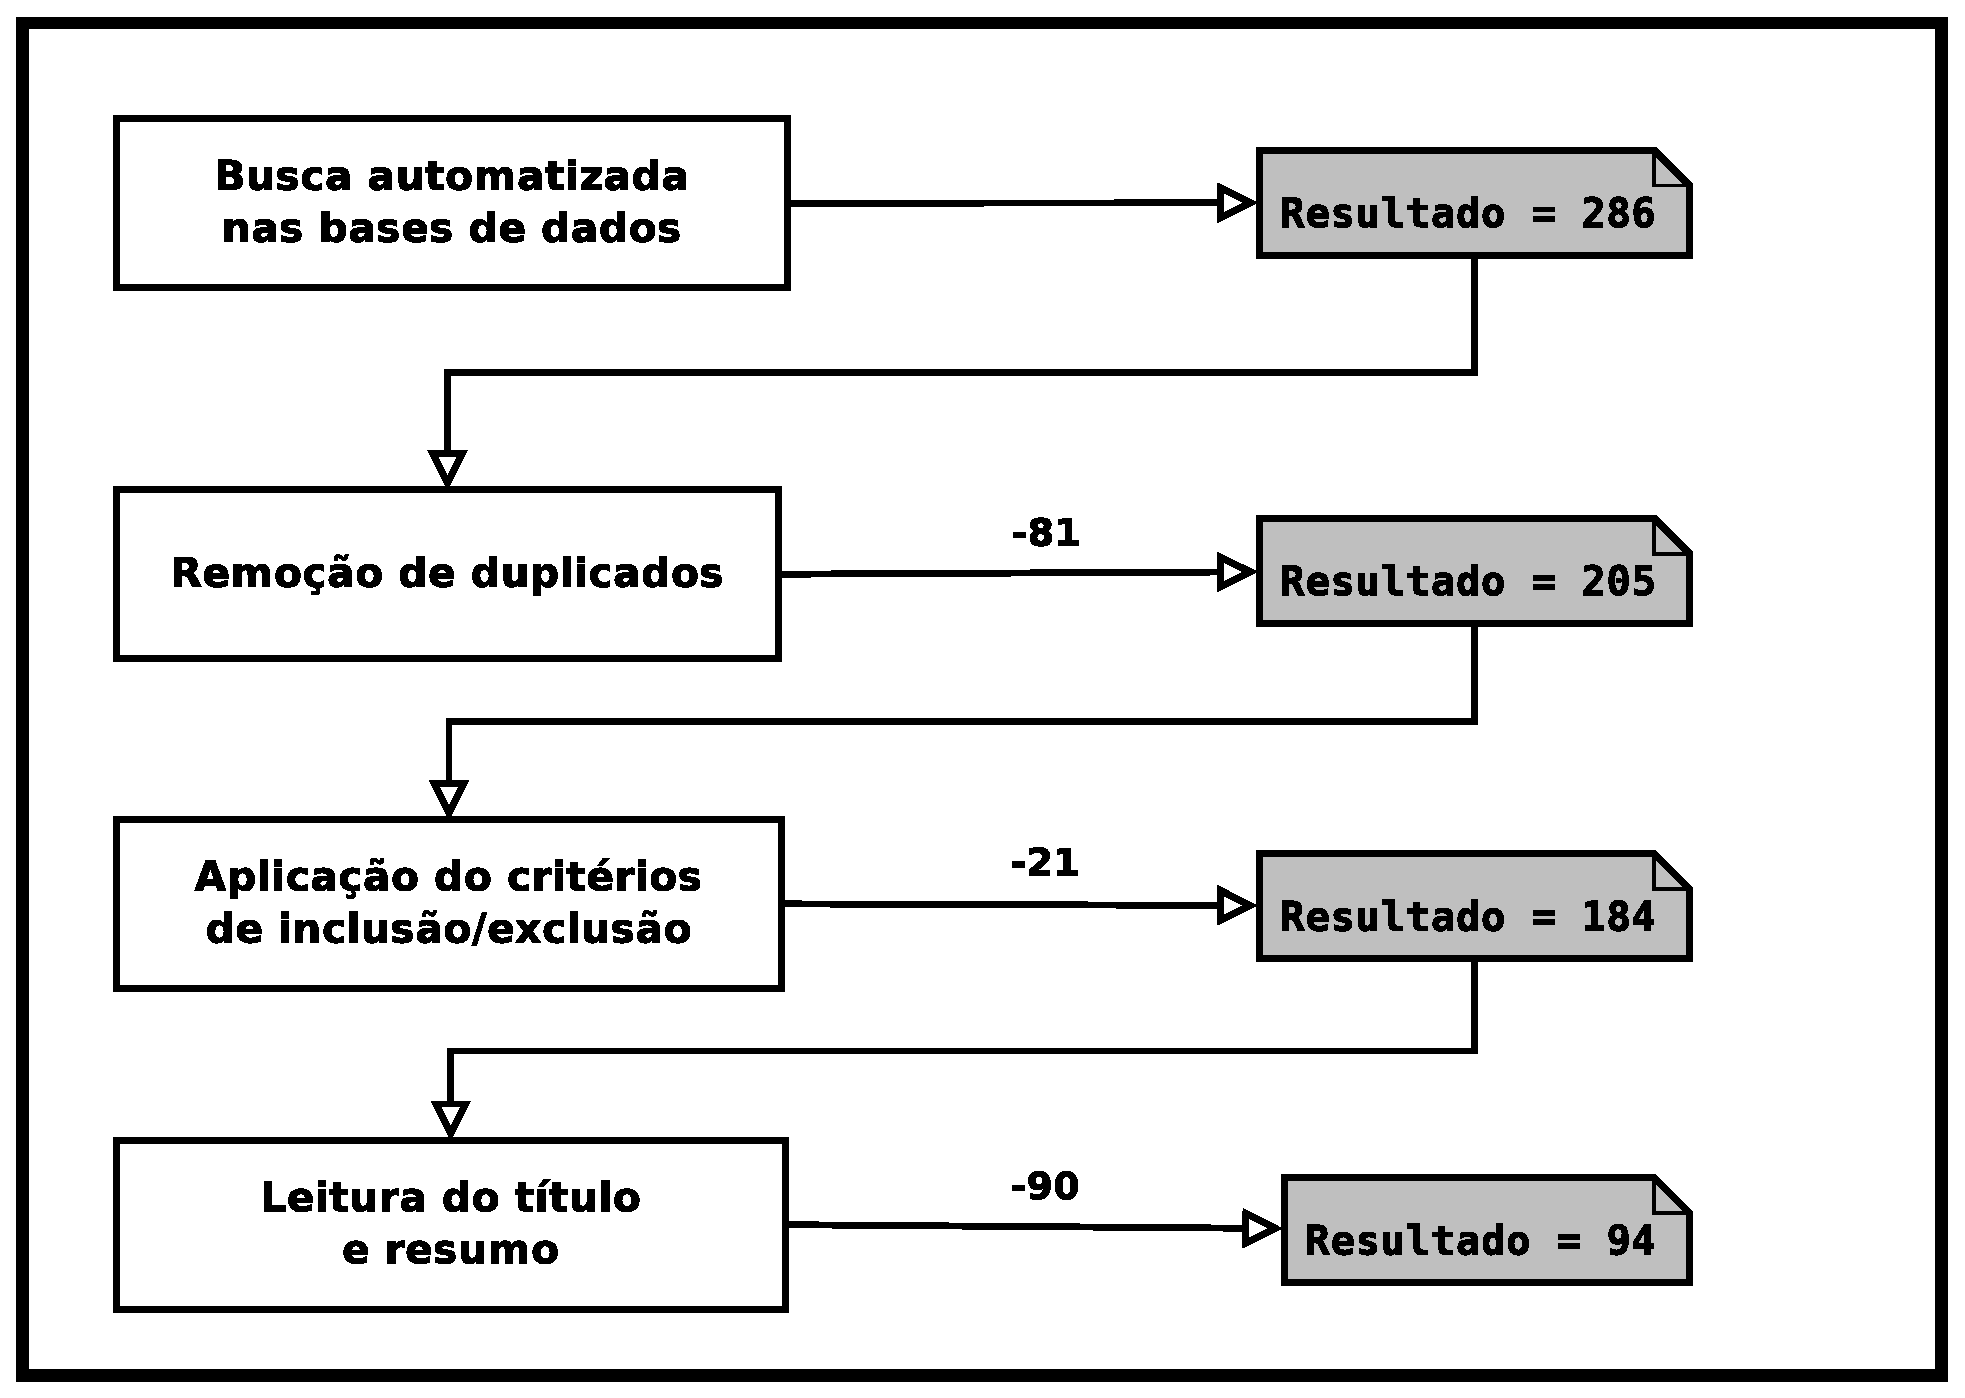
\includegraphics[width=0.75\linewidth]
	{./chapter-mapeamento-sistematico/img/diagrama-processo-selecao.pdf}
	\caption{Número de artigos incluídos durante o processo de seleção dos
		estudos. Figura baseada em~\cite{Petersen2015}}
\label{fig:diagrama-processo-selecao}
\end{figure}

\begin{table}[htb]
	\centering
	\begin{tabular}{cc}
		\toprule
		\textbf{Base de Dados} & \textbf{Total} \\
		\midrule
	   	ACM Digital Library & 109\\
	   	IEEE Explore        & 100\\
		Inspec/Compendex    & 22 \\ 
		Scopus              & 55 \\
		\bottomrule
	\end{tabular}
	\caption{Número de Estudos Recuperados por Base de Dados}
\label{tab:estudos-por-base-dados}
\end{table}

\subsection{Esquemas de Classificação}
\label{subsec:map-esquemas-classificacao}

O mapeamento foi conduzido utilizando dois esquemas de classificação. O primeiro
organiza os artigos pela pertinência com a dimensão de melhoria da
funcionalidade proposta. As dimensões de melhorias foram baseadas no trabalho de
Zimmermann e outros cujo objetivo é aperfeiçoar as funcionalidades das FGRMs de
maneira integral~\cite{zimmermann2009improving}. A segunda classificação
distribui os estudos pelo relacionamento com o suporte dado a determinado papel
no processo de manutenção de software. Entendemos que estes dois esquemas nos
fornecem uma visão de como as melhorias das funcionalidades vêm sendo propostas
tanto do ponto de vista de quem desenvolve quanto das diferentes partes
interessadas dos projetos de software. As pró\-xi\-mas subseções discutem com
mais detalhe cada esquema.

\subsubsection{Classificação por Dimensão de Melhoria}
\label{subsubsec:map-esquema-suporte-problema}

Em um estudo sobre o aperfeiçoamento das FGRMs~\cite{zimmermann2009improving},
os autores argumentam que ter informações completas nos relatos de falhas
(Requisição de Mudança), tão logo quanto possível, ajuda os desenvolvedores a
resolver com mais rapidez o problema. Neste mesmo estudo, eles discutem como
melhorar as funcionalidades oferecidas pelas FGRMs de forma integral, ou seja,
que atenda aos diversos contextos em que este tipo software está integrado.

\begin{description}
	\item[Foco na Informação] Estas melhorias focam diretamente na informação
		fornecida pelo reportador da RM\@. Com ajuda da FGRM, o responsável por
		descrever uma falha, por exemplo, poderia ser motivado a coletar mais
		informações sobre o problema. O sistema poderia verificar a validade e
		consistência do que foi repassado pelo Reportador (detalhes sobre este
		papel pode ser encontrado na
		Subseção~\ref{subsec:man_visao_geral_papeis_na_manutencao_de_software}).
	\item[Foco no Processo] Melhorias com foco no processo visam dar suporte às
		atividades de administração focadas na solução das RMs. Por exemplo, a
		triagem de RM, poderia ser automatizada visando acelerar o processo. Um
		outro exemplo de melhoria poderia ocorrer no aumento do entendimento do
		progresso realizado em cada RM ou mesmo fornecer ao usuário afetado por
		uma falha a estimativa do tempo necessário para atendimento (estimativa
		de esforço).
	\item[Foco no Usuário] Nesta dimensão estão incluídos tanto os usuários que
		relatam as RMs (Reportadores) quanto os desenvolvedores responsáveis por
        solucioná-las. Os reportadores podem ser orientados sobre qual
        informação fornecer e como coletá-la. Os desenvolvedores também podem se
        beneficiar de um treinamento sobre qual informação esperar e como esta
        informação pode ser utilizada para solucionar determinada RM\@.
	\item[Foco na Ferramenta] As melhorias centradas na ferramenta são
		discutidas com vistas às funcionalidades das FGRMs\@. Elas podem reduzir
		a complexidade da coleta e fornecimento das informações necessárias para
		solucionar a RM\@. Por exemplo, as FGRMs poderiam ser configuradas para
		automaticamente identificar a cadeia de registros de ativação de funções
        (\textit{stack trace}) e adicioná-la ao erro reportado. A ferramenta
        poderia ainda simplificar o processo de reprodução do erro mediante a
        captura automatizada de tela (\textit{screenshots}).
\end{description}

Para a classificação dos estudos nos esquemas utilizados foi realizado um
processo baseado no trabalho de Petersen e outros~\cite{Petersen2008}, que é
composto por duas etapas:

\begin{enumerate}[I]
	\item análise das palavras-chaves e conceitos que
		identificam as contribuições do estudo por meio da analise do título e
		resumo.
	\item combinações das palavras-chaves para construir um conjunto de
		categorias para classificação dos artigos.
\end{enumerate}

Os autores recomendam que nos casos em que o resumo e o título do estudo não
sejam capazes de caracterizá-lo, as seções de introdução e conclusão também
devem ser analisadas. Para as bases de pesquisa de dados em que era informado
mais de um conjunto de palavras-chaves para um mesmo artigo, utilizamos aquelas
que foram definidas pelos autores. Mediante a aplicação do processo descrito foi
construído o esquema de classificação apresentado na
Figura~\ref{fig:diagrama-esquema-dimensao-melhorias}.

\begin{figure}[tb] \centering
	\makebox[\textwidth]{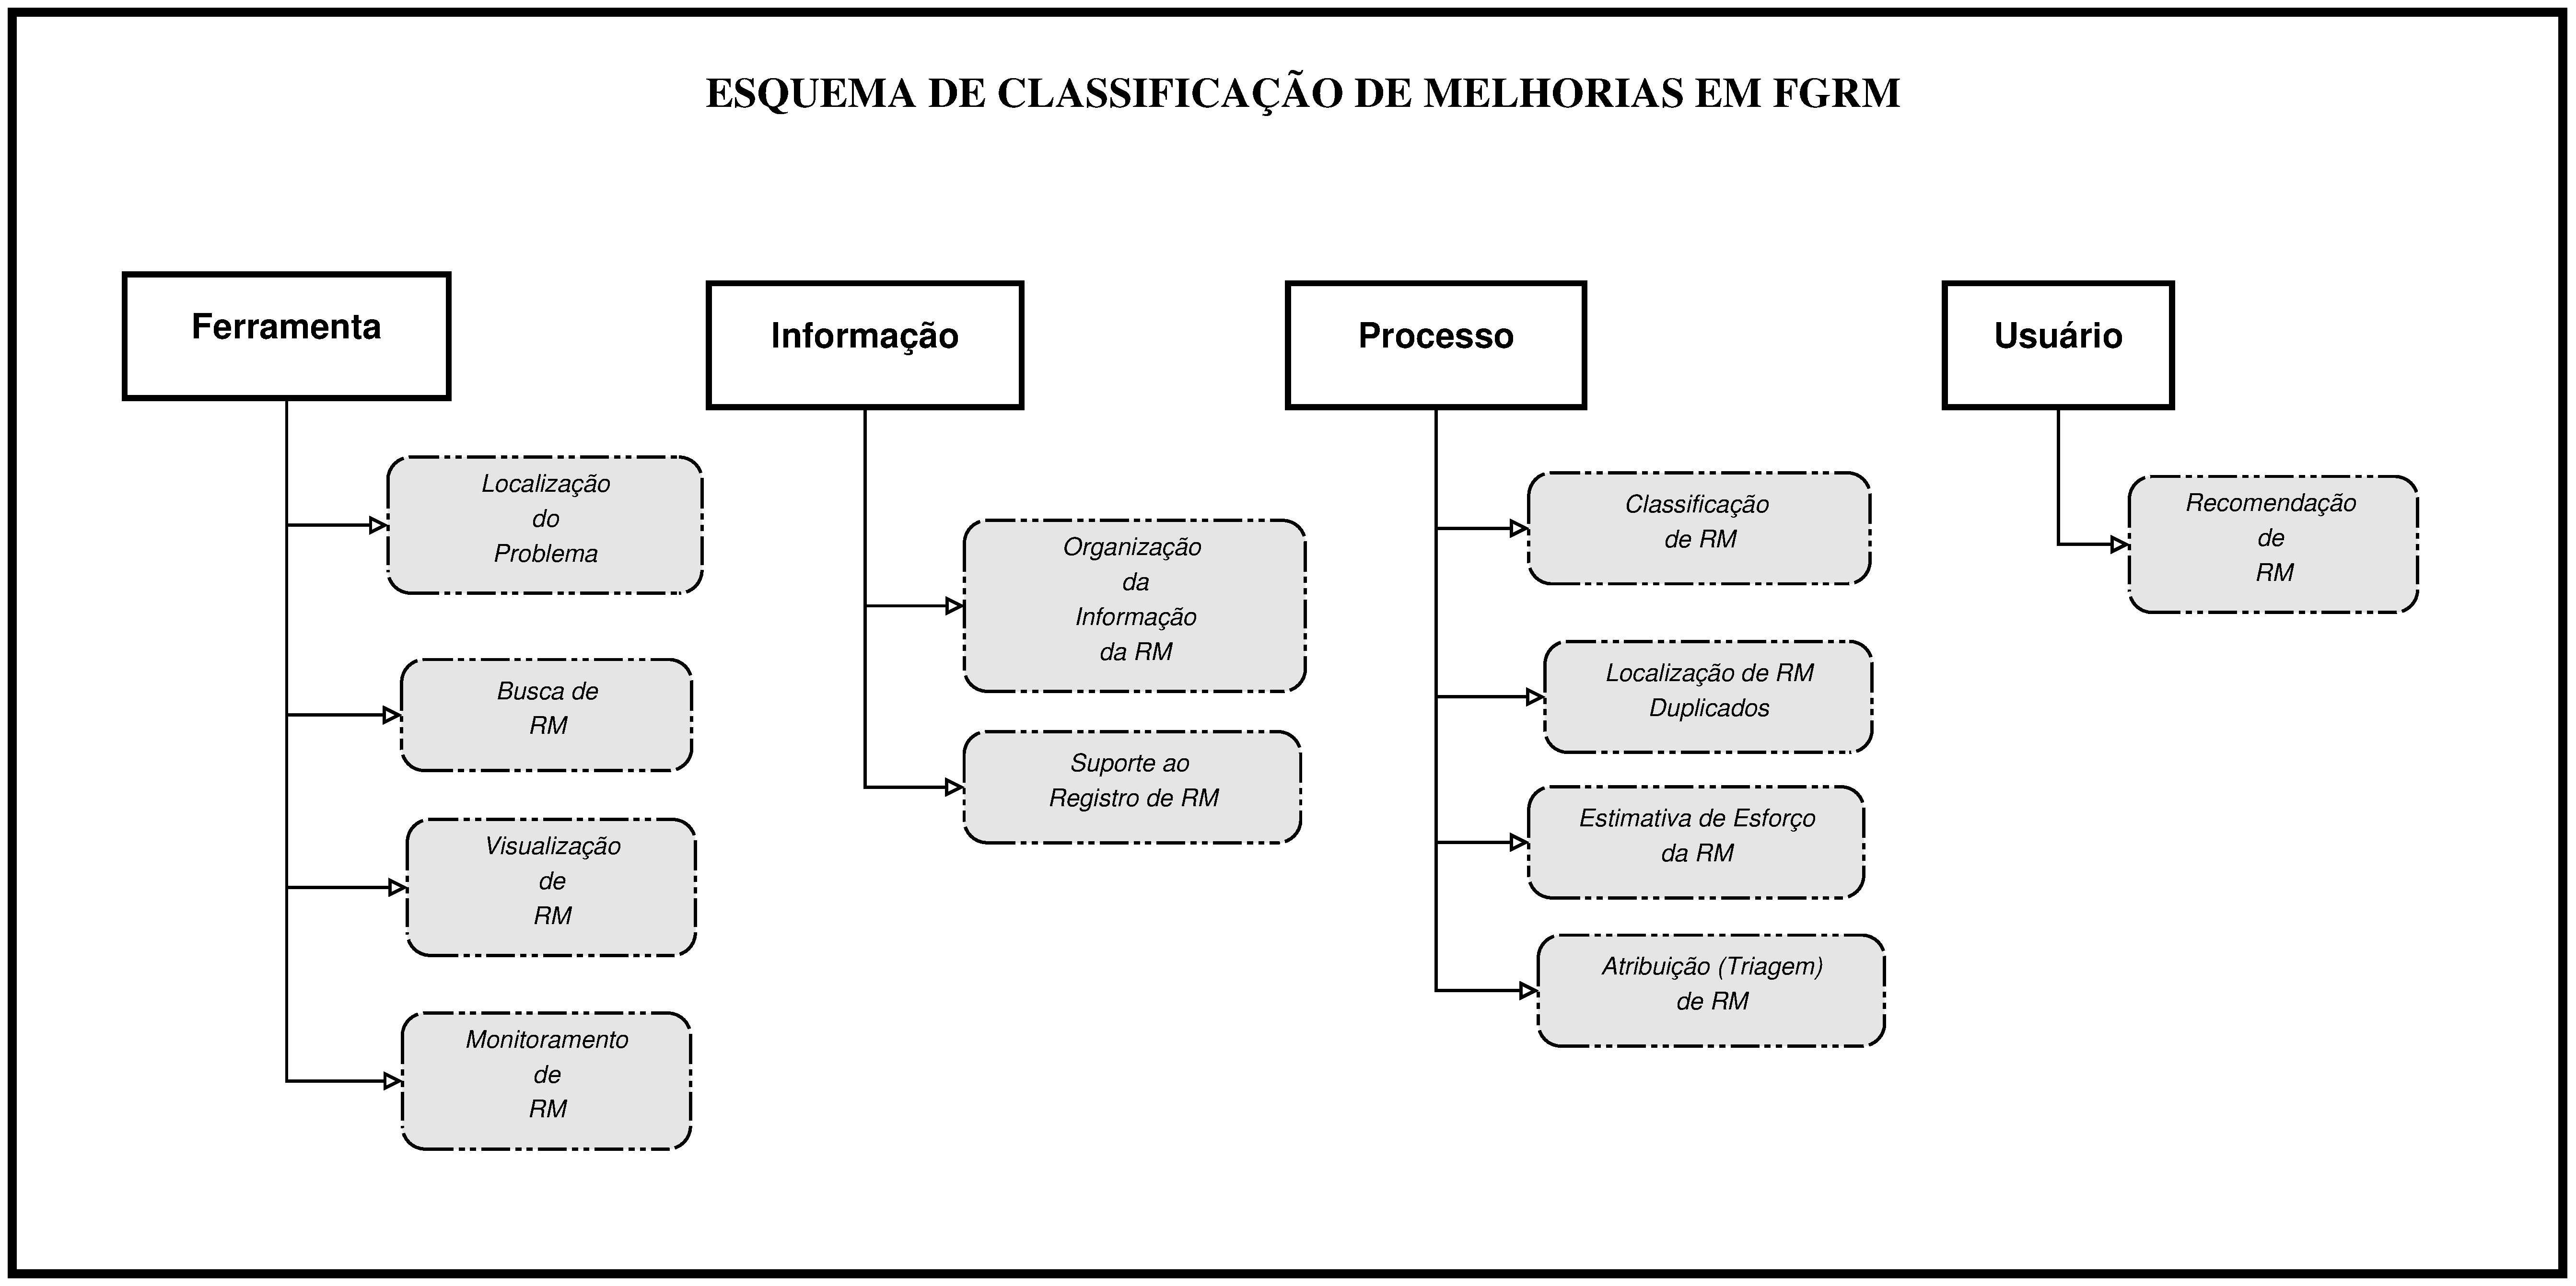
\includegraphics[width=.7\paperwidth]{./chapter-mapeamento-sistematico/img/diagrama-esquema-dimensoes-melhorias.eps}}
    \caption{Esquema de classificação das melhorias propostas na literatura. Os
        retângulos representam as dimensões de melhorias e os polígonos de
        cantos arredondados representam tópicos de problemas do gerenciamento
        das RMs.}
\label{fig:diagrama-esquema-dimensao-melhorias}
\end{figure}

\subsubsection{Classificação por Suporte ao Papel da Manutenção de Software}
\label{subsubsec:map-esquema-suporte-papel-man}

Neste esquema de classificação estamos interessado em avaliar como os estudos
dão suporte aos papéis apresentados na
Subseção~\ref{subsec:man_visao_geral_papeis_na_manutencao_de_software}. A
construção da classificação utiliza a mesma metodologia descrita na seção
anterior e utilizada a classificação de papéis da manutenção proposto por Polo e
outros~\cite{Polo1999}.

\section{Resultados}
\label{sec:mapeamento_resultados}

Nesta seção apresentamos os estudos divididos para cada um dos esquemas de
classificação utilizados. Iniciamos com uma análise da frequência de publicação
sobre o tema do mapeamento e posteriormente apresentamos os resultados para cada
uma das dimensões de melhoria. Seguimos com a análise dos estudos pelo papel ao
qual a funcionalidade proposta visa dar suporte.

A frequência de publicação dos estudos teve em 2010, primeiro ano do período
analisado, um total de 05 trabalhos publicados. A maior quantidade de
publicação ocorreu entre os anos de 2012, 2013 e 2014, com, respectivamente,
14, 12 e 13 artigos. No ano de 2016, último ano do período de referência,
encontramos 03 estudos publicados. A Tabela~\ref{tab:publicacao_por_ano} exibe
o número de estudos primários identificados entre os anos de 2010 e 2016,
período de referência utilizado no mapeamento.

\begin{table}[htpb]
\centering
\resizebox{.25\textwidth}{!}{%
\begin{tabular}{@{}lc@{}}
\toprule
\textbf{Ano} & \textbf{Frequência} \\ \midrule
2010         & 5                   \\
2011         & 8                   \\
2012         & 14                  \\
2013         & 12                  \\
2014         & 13                  \\
2015         & 9                   \\
2016         & 3                   \\ \bottomrule
\end{tabular}%
}
\caption{Número de estudos primários por ano de publicação.}
\label{tab:publicacao_por_ano}
\end{table}

\subsection{Classificação por Dimensões de Melhoria}
\label{sub:extensões_para_problemas_na_manutenção_de_software}

Nesta seção apresentamos estudos relacionados com a dimensão denominada
``Melhoria das funcionalidades das FGRMs\@''. A classificação está estruturada
de modo que no primeiro nível temos uma das quatro dimensões de melhorias
discutidas na Subseção~\ref{subsubsec:map-esquema-suporte-problema}. O segundo
nível é composto por tópicos que são os problemas do gerenciamento das RMs. Uma
discussão mais detalhada sobre estes problemas pode ser encontrada na
Subseção~\ref{ssub:problemas_relacionadas_rm}. A
Tabela~\ref{tab:taxonomia-problemas-manutencao} exibe a distribuição dos
estudos pela dimensão de melhoria e o seu respectivo tópico.

% Inclusão da tabela
% 
\begin{table}[htpb]
\centering
\caption{Taxonomia por Problemas na Manutenção de Software}
\label{tab:taxonomia-problemas-manutencao}
\resizebox{\textwidth}{!}{%
\begin{tabular}{cclc}
\hline
\multicolumn{2}{c}{\textbf{Taxonomia}}
& \multicolumn{1}{c}{\textbf{Artigos}}                                    &
\textbf{Total} \\ \hline
\multirow{3}{*}{\textit{Classificação de Requisições de Mudança}} &
\textit{Duplicação}                &
\cite{alipour2013contextual,hindle2016contextual,sun2010discriminative} & 3
\\
                                                                  &
\textit{Categorização}             & \cite{behl2014bug, zhang2011bug,
chawla2015automated}                   & 3              \\
                                                                  &
\textit{Estimativa de Esforço}     & \cite{hosseini2012market}
& 1              \\ \hline
\textit{Atribuição de Requisições de Mudança}                     &
\textit{Alocação Automática}       & \cite{hosseini2012market}
& 1              \\ \hline
\textit{Resolução de Requisições de Mudança}                      &
\textit{Alocação de Tarefas}       & \cite{netto2010automated}
& 1              \\ \hline
\multirow{2}{*}{\textit{Visualicação de Requisições de Mudança}}  &
\textit{Visualização de Atributos} & \cite{dal2013closer}
& 1              \\
                                                                  &
\textit{Monitoramento}             & \cite{takama2013application}
& 1              \\ \hline
\end{tabular}%
}
\end{table}


\subsubsection{Melhorias Propostas na Dimensão Ferramenta}
\label{ssub:melhorias_dim_ferramenta}

Este ramo do esquema de classificação inclui os estudo que possuem relação com
tópicos como Localização do Problema e Visualização de RMs.

\paragraph{Localização do Problema:}

Os estudos incluídos neste tópico focam em localizar a origem de um problema de
software com base nos dados da RM~\cite{Hovemeyer:2004:FBE:1052883.1052895}.
Com objetivo de melhorar a eficiência da localização de um problema, diversas
informações contidas nas RMs estão sendo utilizadas. As abordagens propostas
utilizam informações como cadeia de registros de
ativação~\cite{Wong:2014:BBF:2705615.2706096}, des\-cri\-ção e campos
estruturados das RMs~\cite{Thung:2014:BIT:2635868.2661678} e os históricos de
versões do código fonte do
sistema~\cite{Bangcharoensap:2012:LSC:2419061.2419428, corley2011recovering,
    Romo:2015:TAT:2745802.2745833}. Algumas das melhorias propostas foram
incluídas em ferramentas largamente empregadas no mercado utilizando os
mecanismos de extensão que elas oferecem. A ferramenta
\textit{BugLocalizer}\footnote{\url{https://github.com/smagsmu/buglocalizer}},
implementada como extensão do Bugzilla, extrai o texto do sumário e do relato
de uma RM e calcula a semelhança entre o texto relatado e o código fonte para
encontrar os arquivos onde a falha possívelmente está
localizada~\cite{Thung:2014:BIT:2635868.2661678}. A ferramenta
\textit{BugTrace}~\cite{corley2011recovering} é uma extensão do Bugzilla que
implementa uma abordagem que analisa os \textit{patches}\footnote{Um
    \textit{patch} é um software projetado para atualizar um programa de
    computador ou seus dados de suporte, para corrigi-lo ou melhorá-lo.}
inseridos em RM para determinar um elo de rastreabilidade entre uma falha e o
código fonte.

\paragraph{Visualização de RM:}

Os estudos neste tópico estão relacionados com melhoria da visualização da
informação contida na RM\@. Com o objetivo de apresentar diferentes formas de
visualizar os dados de uma RM novos conceitos estão sendo propostos. No estudo
de Hora e outros~\cite{hora2012bug} é apresentado o conceito de Mapas de
Defeitos (\textit{BugsMaps)} que mostra a RM e uma ligação dela com outros
artefatos de software, por exemplo, o histórico de versões. O conceito de
hiperligação entre documentos é utilizado para permitir a navegação entre os
artefatos que estão relacionados a uma RM~\cite{dal2014bug}.

Verificamos ainda no artigo proposto por Takama e
Kurosawa~\cite{takama2013application} a aplicação de tecnologias de
visualização de informação empregada para o monitoramento das informações
contidas nas RMs. Uma FGRM atualiza quase toda informação de uma RM como texto,
sem maiores estruturações. A solução proposta pelos autores visa suportar o
monitoramento das RMs apresentando ao usuário da FGRM, seja ele o afetado por
uma falha, o responsável por relatar a requisição ou mesmo um membro da equipe
de manutenção, a situação das RMs mediante animações produzidas com base nas
atualizações ocorridas nas mesmas.

Por conta da natureza das melhorias propostas neste tópico de pesquisa,
verificamos que diversos estudos foram implementados como protótipos. Desta
forma, é possível avaliar as propostas contidas neste tópico através das
ferramentas como o
\textit{bugMaps}\footnote{\url{http://rmod.lille.inria.fr/web/pier/software/BugMaps}}~\cite{hora2012bug}
e \textit{In* Bug}\footnote{\url{http://inbug.inf.usi.ch}}~\cite{dal2014bug}.

\subsubsection{Melhorias Propostas na Dimensão Informação}
\label{ssub:melhorias_dim_informacao}

Apresentamos os trabalhos relacionados à melhoria da qualidade da informação de
uma RM\@. A melhoria pode envolver suporte ao registro de uma RM antes que ela
seja armazenada no Repositório de RMs; a melhoria também pode envolver a
organização da informação contida no relato para facilitar o entendimento pelos
desenvolvedores e demais profissionais envolvidos na manutenção de software.

\paragraph{Suporte ao Registro da RM:}

Para melhorar a qualidade da informação fornecida nas RMs os artigos sobre o
tema, em sua maioria, definem um limiar para algum atributo do texto
correspondente ao relato da RM\@. Caso este limiar não seja alcançado alguma
ação é tomada, como por exemplo, a exibição de uma mensagem de alerta para o
responsável pela criação da RM\@. A determinação do que seria um boa descrição
de um problema de software foi obtida mediante uma pesquisa com profissionais
envolvidos com manutenção de software no estudo de Bettenburg e
outros~\cite{bettenburg2008makes}. Em outro estudo os próprios autores definiram
as métricas que posteriormente foram utilizadas para avaliar o relato da
RM~\cite{Tu:2014:MQI:2677832.2677844}.

Um segundo nicho de estudos visa suportar a reprodução da falha do software.
Estes estudos incluem tanto registrar o conjunto de ações que resultaram na
falha~\cite{White:2015:GRR:2820282.2820291}, quanto em autocompletar o texto que
compõe o relato de uma falha~\cite{moran2015auto}. Um ponto em comum deste dois
estudos é que eles foram pensados para o ambiente de desenvolvimento de
aplicações para dispositivos móveis, mais especificamente para dispositivos
baseados no sistema Android\footnote{\url{https://www.android.com/}}. Uma
possível justificativa para o foco em aplicações móveis pode ser a dificuldade
em registrar uma falha neste tipo de
ambiente~\cite{White:2015:GRR:2820282.2820291, moran2015auto}.

Muitos dos estudos resultaram em ferramentas com a finalidade de realizar uma
prova de conceito sobre como ajudar ao Reportador a fornecer um relato de boa
qualidade~\cite{Tu:2014:MQI:2677832.2677844, bettenburg2008makes,
    Wu2011a,White:2015:GRR:2820282.2820291,moran2015auto}.

\paragraph{Organização da Informação da RM:}

Em diversas situações o desenvolvedor precisa examinar manualmente o relato das
RMs que podem variar em tamanho e complexidade~\cite{mani2012ausum}. Neste
contexto, o resumo (sumarização) automático do texto contido em uma RM é uma
maneira de reduzir a quantidade de dados que o desenvolvedor precisa analisar.
A ferramenta denominada AUSUM~\cite{mani2012ausum} propõe uma abordagem,
utilizando técnicas não supervisionadas de aprendizado de máquina, para aprender
e sumarizar um ou mais relatos relacionados.

\subsubsection{Melhorias Propostas na Dimensão Processo}
\label{ssub:melhorias_dim_processo}

\paragraph{Identificação de RMs Duplicadas}

O processo de identificação de RMs duplicadas consiste em avaliar se
determinado relato já foi realizado em algum outro momento.  A literatura
discute dois tipos de tratamento para o problema~\cite{kaushik2012comparative,
    Tian2012}:

\begin{enumerate}[(i)]

	\item remoção de duplicadas

	\item identificação de duplicatas

\end{enumerate}

No primeiro tipo, o objetivo é evitar que RMs duplicadas entrem no repositórios
de RMs e, desta forma, evitar o esforço e o tempo extra necessário para
identificá-las posteriormente. Por outro lado, no segundo tipo o objetivo é
sugerir uma lista de possíveis duplicatas durante o processo de registro de uma
nova RM\@. Um ponto importante é que o segundo tipo se baseia na premissa que
registrar um mesmo problema por mais de uma vez nem sempre é ruim, já que a
possível ``cópia'' pode fornecer informações
adicionais~\cite{bettenburg2008duplicate}. É importante que novas abordagens
tentem equilibrar estes dois tipos de tratamento para evitar o tempo extra para
análise de uma RM bem como apoiar os desenvolvedores com informações
adicionais~\cite{Lerch:2013:FDY:2495256.2495763,Thung2014}.

Uma forma de tratar o problema é utilizar modelos de espaços vetoriais para
medir a similaridade entre as RMs~\cite{liu2014faceted, sun2010discriminative,
    Thung2014,tomavsev2013exploiting}. Outros trabalhos tentam utilizar técnicas
em que os termos específicos do domínio do projeto de software, contidos no
relato das RMs, são utilizados na determinação da probabilidade que duas
requisições sejam duplicadas~\cite{hindle2016contextual, alipour2013contextual}.
Em resumo verificamos que o relato contido na RM é utilizado como fonte de
informação para técnicas de Re\-cu\-pe\-ra\-ção da Informação visando determinar
a similaridade entre duas RMs.

\paragraph{Atribuição (Triagem) de RM:}

Os estudos apresentados neste tópico foram classificados pela pertinência com a
automatização do processo de encontrar o desenvolvedor mais apto para solucionar
determinada RM\@. A principal fonte de informação utilizada nas abordagens
propostas é o relato contido na RM, todavia, outros dados são utilizados, tais
como a prioridade~\cite{tian2015automated}, registros (log) do sistema de
controle de versão~\cite{shokripour2012automatic, Hu:2014:EBT:2707683.2708297} e
itens do contexto do projeto como por exemplo: o perfil e preferências do
desenvolvedor, quantidade de RMs atribuídas e o tempo estimado de
correção~\cite{hosseini2012market}. Em outros trabalhos verificamos que é
explorada a característica colaborativa que existe no processo de triagem das
RMs. Nestes estudos é desenvolvida uma ``rede de colaboração'' que possibilita
determinar o desenvolvedor mais apto~\cite{Zhang2014,Zanetti2013, Wu2011}.  Em
geral técnicas de Recuperação da Informação (RI) são utilizadas pelos estudos
que espaço vetorial e ranqueamento de páginas.

\paragraph{Classificação da RM:}

Os estudos neste tópico visam automatizar o processo de clas\-si\-fi\-ca\-ção
de uma RM\@.  Este tipo de abordagem faz uso da funcionalidade de atribuição de
rótulo (\textit{labels}) que é comum  a grande parte das FGRMs. Em muitos
projetos esta atividade é realizada manualmente pelo Agente de Triagem,
Desenvolvedor ou Analista de Qualidade, o que pode resultar em classificações
equivocadas.

Esta classificação pode ser realizada pelo tipo de manutenção (Corretiva,
Adaptativa, Perfectiva e Preventiva), se a RM trata de questões relativas à
segurança do sistema~\cite{gegick2010identifying, behl2014bug} ou pelo nível de
prioridade que a requisição deve ser analisada~\cite{behl2014bug}.

\paragraph{Estimativa de Esforço da RM:}

Identificamos três tipos de estimativas de esforço relacionadas a uma RM\@:
determinar o tempo para solucionar novas RMs; definir os artefatos que são
impactados pela RM\@; prever o número de RMs que poderão surgir em futuras
versões do sistema. Nos estudos que tratam da primeira forma de estimativa a
preocupação é o tempo necessário para tratar a mudança solicitada em determinada
requisição. A principal complexidade está em produzir uma estimativa precisa em
função das muitas atividades envolvidas e dos diferentes níveis de capacitação
do responsável pela execução das tarefas~\cite{xia2015automatic}. No segundo
grupo temos os artigos que tentam identificar previamente o conjunto de
artefatos que serão impactados pela tarefa de manutenção~\cite{Nagwani2010}.
Neste mapeamento o foco foi em estudos em que as RMs são o ponto de partida para
a análise de impacto. O último grupo de estudos discute técnicas sobre como
prever o número de RMs que possivelmente serão incluídas em futuras versões do
sistema. A predição do que será registrados inclui RMs que não existiam em
versões anteriores como aquelas que serão reabertas, ou seja, problemas que não
foram solucionados previamente~\cite{xia2015automatic}.

\subsubsection{Melhorias Propostas na Dimensão Usuário}
\label{ssub:melhorias_dim_usuario}

\paragraph{Recomendação de RM:}

Os estudos deste tópico dão suporte aos desenvolvedores com pouca experiência
mediante a redução da curva de aprendizagem. Para facilitar a inclusão
desenvolvedores menos experientes alguns estudos propõem sistemas de
recomendação de RMs~\cite{malheiros2012source, Wang2011bug}. Estes sistemas
podem ajudar o recém-chegado a solucionar uma RM mediante a apresentação do
código fonte potencialmente relevante que o ajudará na solução do
problema~\cite{malheiros2012source}. O segundo tipo de abordagem pode ser vista
como ambiente de exploração do repositório de RMs. Esta funcionalidade permite
que novos desenvolvedores pesquisem descrições das requisições que possam ser do
seu interesse bem como dos artefatos relacionados (por exemplo, arquivos
relacionados, desenvolvedores contribuintes, registros de
comunicação)~\cite{Wang2011bug}. Com base nos estudos que compõem esta
categoria, verificamos que modelos de RI vêm sendo utilizados para possibilitar
a recomendação das RMs\@, tais como VSM~\cite{Wang2011bug} e o modelo
estatístico PPM~\cite{malheiros2012source}.

\subsection{Suporte à Papéis da Manutenção de Software}
\label{sub:extensões_com_suporte_a_papeis}

Nesta subseção são discutidos os estudos que foram considerados relacionados
com papeis abordados na
Subseção~\ref{subsec:man_visao_geral_papeis_na_manutencao_de_software}. A
Tabela~\ref{tab:graf_papel_por_artigo} exibe o total de artigos por papel que a
funcionalidade proposta visa dar suporte.  Como pode ser observado verificamos
um maior número de estudos para os papéis de Agente de Triagem e Desenvolvedor.
Na Tabela~\ref{tab:taxonomia-suporte-papeis} é possível observar os estudos
pelo papel o qual dão suporte. É possível observar que um mesmo estudo pode dar
suporte a mais de um papel. Por exemplo, o estudo de Bettenburg e outros
propõe uma ferramenta que mede a qualidade do relato das RMs e recomenda quais
elementos devem ser adicionados para melhorar a
qualidade~\cite{bettenburg2008makes}. Os possíveis benefícios podem ajudar o
\textit{Reportador}, que pode ter reduzido o tempo para analisar a RM que ele
registrou já que a RM fornece a informação necessária para sua análise; o
\textit{Desenvolvedor}, que recebe uma RM com mais qualidade nos dados
fornecidos; o \textit{Analista de Qualidade} que consegue avaliar se a RM foi
atendida tendo em vista a maior facilidade em entender o que foi solicitado.

\begin{table}[htpb]
\centering
\resizebox{.6\textwidth}{!}{%
\begin{tabular}{lc}
\toprule
\multicolumn{1}{c}{\textbf{Papel}} & \textbf{Total de Artigos} \\
\midrule
Agente de Triagem & 37 \\
Desenvolvedor & 26 \\
Analista de Qualidade & 13 \\
Gerente de Requisição de Mudança & 11 \\
Reportador & 6 \\
Líder da Manutenção & 4 \\
Todos & 3 \\
\bottomrule
\end{tabular}%
}
\caption{Total de artigos por papel na manutenção de software}
\label{tab:graf_papel_por_artigo}
\end{table}

% Inclusão da tabela do suporte dos papéis
\begin{table}[htbp]
\centering
\resizebox{1.15\textwidth}{!}{%
\begin{tabular}{@{}cl@{}}
\toprule
\textbf{Papel Suportado} & \multicolumn{1}{c}{\textbf{Estudos}} \\ \midrule
\multirow{9}{*}{\textit{Atribuidor}} & \cite{banitaan2013decoba, gegick2010identifying,izquierdo2015gila, liu2014faceted} \\
 & \cite{nagwani2013generating, behl2014bug, chawla2015automated, hosseini2012market} \\
 & \cite{mani2012ausum, Sun2011, tian2015automated, shokripour2012automatic} \\
 & \cite{Bhattacharya:2011:BTP:1985441.1985472,  Wu2011a, Naguib2013, Zhang2014, Zanetti2013} \\
 & \cite{ValdiviaGarcia:2014:CPB:2597073.2597099, Koopaei:2015:CAD:2886444.2886474, Prifti2011, Xuan:2012:DPB:2337223.2337227} \\
 & \cite{Wu2011, Thung2014, tian2013drone, Lerch:2013:FDY:2495256.2495763, tomavsev2013exploiting} \\
 & \cite{White:2015:GRR:2820282.2820291, Tian2012, Song2010a, Bangcharoensap:2012:LSC:2419061.2419428} \\
 & \cite{Aggarwal:2014:MIT:2593801.2593810, Nagwani2012, Nagwani2010, Tu:2014:MQI:2677832.2677844} \\
 & \cite{Hu:2014:EBT:2707683.2708297, otoom2016severity} \\ \midrule
\multirow{3}{*}{\textit{Analista de Qualidade}} & \cite{izquierdo2015gila,
    gegick2010identifying, Aggarwal:2014:MIT:2593801.2593810,
    zimmermann2010makes} \\
 & \cite{corley2011recovering, Song2010a, Nguyen:2012:MAR:2393596.2393671, White:2015:GRR:2820282.2820291} \\
 & \cite{thung2012would, xia2015automatic, Tu:2014:MQI:2677832.2677844, Romo:2015:TAT:2745802.2745833, White:2015:GRR:2820282.2820291} \\ \midrule
\multirow{7}{*}{\textit{Desenvolvedor}} &
\cite{White:2015:GRR:2820282.2820291,zimmermann2010makes, Thung:2014:BIT:2635868.2661678, Nguyen:2012:MAR:2393596.2393671} \\
 & \cite{Wang2011bug, Romo:2015:TAT:2745802.2745833, ValdiviaGarcia:2014:CPB:2597073.2597099, Nagwani2010} \\
 & \cite{Koopaei:2015:CAD:2886444.2886474, Prifti2011, thung2012would, White:2015:GRR:2820282.2820291} \\
 & \cite{tomavsev2013exploiting, thung2013automatic, banitaan2013decoba, corley2011recovering} \\
 & \cite{Vijayakumar2014, gegick2010identifying, izquierdo2015gila, Tian2012} \\
 & \cite{malheiros2012source, Song2010a, mani2012ausum} \\
 & \cite{Tu:2014:MQI:2677832.2677844, Aggarwal:2014:MIT:2593801.2593810, Wong:2014:BBF:2705615.2706096} \\ \midrule
\multirow{3}{*}{Gerente de Requisição de Mudança} & \cite{Vijayakumar2014, mani2012ausum, hindle2016contextual} \\
 & \cite{gegick2010identifying, sun2010discriminative, alipour2013contextual, zhang2011bug} \\
 & \cite{Nagwani2010, kochhar2014automatic, banerjee2012automated, ValdiviaGarcia:2014:CPB:2597073.2597099} \\ \midrule
Líder da Manutenção & \cite{Vijayakumar2014, Tian2012, netto2010automated, Nagwani2010} \\ \midrule
\multirow{2}{*}{Reportador} & \cite{zimmermann2010makes, Tu:2014:MQI:2677832.2677844, Vijayakumar2014} \\
 & \cite{Moran:2015:EAA:2786805.2807557, Thung2014, moran2015auto} \\ \midrule
Todos & \cite{hora2012bug, takama2013application, dal2014bug} \\ \bottomrule
\end{tabular}%
}
\caption{Lista de artigos de acordo com o papel suportado}\label{tab:taxonomia-suporte-papeis}
\end{table}

\paragraph{Agente de Triagem:}

Esta função tem como principal objetivo a atribuição das RMs para o
desenvolvedor mais apto~\cite{banitaan2013decoba}.  Os estudos recuperados
focam em apresentar soluções de atribuição automática~\cite{banitaan2013decoba,
    shokripour2012automatic, somasundaram2012automatic, Naguib2013, Zhang2014,
    Zanetti2013}; classificação
automatizada~\cite{gegick2010identifying,liu2014faceted, behl2014bug,
    chawla2015automated,tian2015automated}; visualização das RMs armazenadas no
repositórios de RMs~\cite{izquierdo2015gila}; agrupamento (clustering) das
requisições~\cite{liu2014faceted}; identificação do tempo necessário para
solucionar a RM (\textit{time to fix})~\cite{hosseini2012market,
    Bhattacharya:2011:BTP:1985441.1985472}; sumarização da informação contida
na RM~\cite{mani2012ausum}; determinação de RMs duplicadas~\cite{Sun2011,
    Wu2011a}.

\paragraph{Desenvolvedor:}

Apresentamos aqui os trabalhos com foco em aspectos de co\-di\-fi\-ca\-ção,
depuração e testes. No suporte ao desenvolvedor identificamos estudos que
propõem a atribuição de RMs a um conjunto de desenvolvedores, em contraposição
da tradicional atribuição a um único desenvolvedor~\cite{banitaan2013decoba},
visando minimizar os pro\-ble\-mas decorrentes da propriedade de código e
propiciar um maior nivelamento de informações entre os membros da equipe. Não
obstante, o maior grupo de estudos nesta categoria está relacionado com a ajuda
ao desenvolvedor na vinculação de determinado problema do software à sua efetiva
origem, que nesta dissertação foi denominado como Localização do
Problema~\cite{corley2011recovering,Wong:2014:BBF:2705615.2706096,
    Thung:2014:BIT:2635868.2661678,Nguyen:2012:MAR:2393596.2393671,thung2013automatic,
    Romo:2015:TAT:2745802.2745833}. Nesta mesma categoria verificamos estudos
que dão suporte ao desenvolvedor na classificação da RM que lhe foi atribuída,
em especial aquelas que estão relacionadas às questões de segurança do
sistema~\cite{gegick2010identifying} ou aquelas que impedem a resolução de
outras (\textit{blocking-bugs})~\cite{ValdiviaGarcia:2014:CPB:2597073.2597099}.

\paragraph{Analista de Qualidade:}

Cabe ao Analista de qualidade avaliar se uma RM considerada ``solucionada'' por
um desenvolvedor foi corretamente resolvida. De maneira similar ao que ocorre
nos estudos que estão relacionados com o tópico de classificação
``Desenvolvedor'' verificamos uma prevalência dos estudos com foco no apoio para
encontrar o defeito no código fonte a partir do relato da falha durante execução
do software~\cite{corley2011recovering,Wong:2014:BBF:2705615.2706096,
    Thung:2014:BIT:2635868.2661678,Nguyen:2012:MAR:2393596.2393671,thung2013automatic,
    Romo:2015:TAT:2745802.2745833}. Verificamos ainda estudos que tentam
predizer a probabilidade que determinada RM será
reaberta~\cite{xia2015automatic}, o que pode ajudar ao Analista de Qualidade na
priorização das requisições com alta possibilidade de reabertura.

\paragraph{Gerente de Requisição de	Mudança:}

O papel que representa esta classe está vinculado ao gerenciamento do processo
de manutenção de software, em especial por decidir se uma RM será aceita ou
rejeitada. As melhorias relacionadas à classificação quanto ao
nível de segurança~\cite{gegick2010identifying, zhang2011bug,
    ValdiviaGarcia:2014:CPB:2597073.2597099}, identificação de
duplicadas~\cite{hindle2016contextual, sun2010discriminative,
    alipour2013contextual, banerjee2012automated} pode ajudar no desempenho
desta atividade.

\paragraph{Reportador:}

Os estudos que fazem parte desta categoria  partem da premissa que melhorar a
qualidade da informação fornecida na RM é o ponto de partida para tratar outros
problemas relacionados ao processo de manutenção de
software~\cite{moran2015auto, Moran:2015:EAA:2786805.2807557,
    bettenburg2008makes}.  Neste sentido verificamos trabalhos para
autocompletar as informações fornecidas pelo Reportador~\cite{moran2015auto},
suporte à reprodução do problema~\cite{Moran:2015:EAA:2786805.2807557}; análise
da qualidade da informação fornecida~\cite{bettenburg2008makes,
    Tu:2014:MQI:2677832.2677844}.  Esta categoria também contempla um estudo que
verifica se o problema relatado já foi registrado~\cite{Thung2014}.

\paragraph{Chefe da Manutenção:}

O Chefe da Manutenção tem por responsabilidade definir os padrões e
procedimentos que compõem o processo de manutenção que será utilizado. Para
ajudar neste trabalho alguns estudos propõem melhorar a alocação de tarefas do
processo de resolução das Requisições de Mudanças~\cite{netto2010automated}.
Outros estudos visam estimar o esforço necessário para solucionar determinada
RM~\cite{Vijayakumar2014, Nagwani2010}, estes aspectos têm o potencial de ajudar
o Chefe de Manutenção no planejamento de liberações de novas versões do sistema
mantido.

\paragraph{Todos:}

Esta categoria abarca os estudos para o qual a melhoria proposta possui impacto
positivo para todos os papéis envolvidos na manutenção de software. A definição
que o foco da melhoria é geral decorre do que foi dito como objetivo dos autores
dos estudos que fazem parte desta categoria ou ainda por não ser possível
determinar uma atividade específica sendo beneficiada.

Conforme pode ser observado, os estudos estão relacionados principalmente com a
melhoria da  visualização das informações contidas nas RMs~\cite{hora2012bug,
	takama2013application, dal2014bug}. Os aperfeiçoamentos podem estar
vinculados a questões de usabilidade das ferramentas, como por exemplo a
navegabilidade entre as RMs~\cite{dal2014bug}.

\section{Discussão}
\label{sec:discussao}

Ao realizarmos este mapeamento verificamos uma prevalência de estudos na
dimensão \textit{Processo} especialmente para os tópicos de \textit{Localização
    de RMs Duplicadas, Atribuição (Triagem) de RMs e Classificação de RMs},
respectivamente. A prevalência destes tópicos pode estar relacionada ao fato de
que eles afetam projetos de diferentes tipos e tamanhos. No caso da
\textit{Localização de RMs Duplicadas} apesar de ser o de maior frequência não é
um problema identificado como o de impacto mais significativo por alguns
desenvolvedores~\cite{bettenburg2008makes}.

Dos estudos que fizeram parte do mapeamento um total de 10 foram implementados
como extensões ou protótipos. No nosso entendimento este número poderia ser
maior a fim de permitir avaliações pelos profissionais envolvidos em manutenção
de software. Cabe ressaltar que no escopo de um estudo pode não estar prevista a
efetiva transformação da melhoria proposta de modo a ser utilizada efetivamente
pelo seu público-alvo, como por exemplo, a criação ou melhoria de uma
funcionalidade em determinada FGRM\@. Além disso, não colocamos como objetivo de
nossa dissertação avaliar ou discutir a facilidade que as FGRMs possuem para
criar novas funcionalidades ou melhorias.

% Contudo, o nosso entendimento é de que um maior número de melhorias propostas na
% literatura sendo utilizadas pelos profissionais envolvidos em manutenção de
% software poderia melhorar a qualidade das soluções mediante a redução da
% diferença entre o estado-da-prática com o estado-da-arte.

Quando analisamos o esquema de Classificação por Papéis, verificamos uma
prevalência de estudos com foco no papel de \textit{Agente de Triagem}. Existe
possivelmente uma crença de que é possível melhorar a produtividade do processo
de manutenção de software reduzindo o esforço de encontrar o desenvolvedor mais
apto. Os estudos que fazem parte desta classe destacam que um considerável
conhecimento sobre o projeto é necessário bem como a capacidade de negociação
com os desenvolvedores e demais partes interessadas são importantes para o
desempenho do papel. Todavia, tendo em vista o esforço e tempo gasto por esta
tarefa, especialmente quando realizada ma\-nu\-al\-men\-te, seria importante que
as FGRMs automatizassem algumas destas atividades. Um outro ponto a destacar é
que as FGRMs deveriam dar suporte ao Reportador que, na maioria da vezes, é o
primeiro a registrar as informações que serão necessárias à solução da RM\@.

\section{Limitações e Ameaças à Validade}
\label{sec:map_limitacoes_ameacas}

Alguns dos procedimentos adotados neste trabalho não acompanharam exatamente as
diretrizes existente na literatura para condução de uma Mapeamento Sistemático.
A seleção dos estudos foi realiza pelo autor sem que outra pessoa fizesse a
revisão. O mapeamento realizado nesta pesquisa utilizou o método de aplicação
de sentenças de busca nas bases de pesquisa selecionadas para coletar os
estudos primários. Outros estudos, além da estratégia descrita, fazem uso de
uma técnica conhecida como
bola~de~neve~(\textit{snowballing})~\cite{wohlin2014guidelines} em que as
referências dos estudos primários podem ser usadas para compor o conjunto de
artigos do mapeamento. O uso de uma única estratégia pode levar a perda de
artigos relevantes e, portanto, subestimar a extensão dos resultados
encontrados. Em particular, por termos optado por escolher artigos apenas em
língua inglesa também pode ter havido falta de material publicado em revistas e
conferências nacionais. Assim, nossos resultados devem ser considerados apenas
com base em artigos em inglês contidos nas bases de pesquisa escolhidas e
publicados nas principais conferências da área de Engenharia de Software.

O fato que o autor foi o único responsável pela análise dos estudos aumenta o
risco de erros. O processo de seleção e validação dos estudos primários pode
levar a problemas de extração e agregação das informações quando há um grande
número de artigos ou os dados são complexos~\cite{keele2007guidelines}. No
entanto, neste estudo secundário, houve poucos estudos primários e os dados
recuperados eram razoavelmente objetivos. Desta forma, não acreditamos em
muitos erros.

No tocante às questões deste estudo é possível que as perguntas de pesquisa
definidas possam não abranger completamente o campo de investigação sobre as
funcionalidades das FGRMs. No entanto, algumas discussões com membros do
projeto e especialistas em Manutenção de Software foram realizadas para validar
as perguntas. Assim, mesmo que não tenhamos considerado o melhor conjunto de
questões, tentamos abordar as indagações mais frequentes e abertas no campo,
tanto do ponto de vista do praticante como do investigador.

Como as bases de pesquisa não funcionam com regras de busca compatíveis entre
si, todas as sequências de pesquisa foram adaptadas e calibradas em cada uma
delas. No entanto, não conhecemos todas as regras que as bases de pesquisa
utilizam para indexar um documento. Neste sentido, a forma que as sentenças de
busca foram estruturadas pode não ser a mais otimizada para pesquisa do maior
número de documentos relevantes.

O nosso estudo considerou publicações até maio de 2016. De lá pra cá verificamos
que assuntos como Identificação de RMs Duplicadas~\cite{aggarwal2017detecting,
    chaparro2017improving, sadat2017rediscovery} e Classificação da
RM~\cite{karim2017understanding, zibran2016effectiveness, ohira2016case} ainda
permanecem entre aqueles com a maior frequência de publicação.

\section{Trabalhos Relacionados}
\label{sec:map_trabalhos_relacionados}

No estudo proposto por Kagdi e outros~\cite{kagdi2012assigning} foi realizada
uma revisão da literatura sobre abordagens para mi\-ne\-ra\-ção de repositórios
de RMs. No contexto daquele trabalho este tipo de repositório pode ser
comparado ao repositório de RMs empregados nas FGRMs. O resultado foi uma
taxonomia baseada em quatro classes: o tipo de repositório extraído (o que), o
propósito (por que), o método proposto (como) e o método de avaliação
(qualidade). No entanto, a sua classificação não fornece um entendimento
extensivo sobre as investigações em repositórios de RMs\@. De acordo com seus
critérios de exclusão para estudos, eles estavam muito preocupados com artigos
que abordavam mudanças evolutivas de artefatos de software investigando
múltiplos repositórios de RMs. Como consequência, muitos trabalhos que usaram
dados de um único repositório de RM estavam fora do seu escopo.

Por outro lado, o estudo realizado neste capítulo aumentou o escopo da análise
sobre as funcionalidades oferecidas pelas FGRMs possibilitando uma visão mais
abrangente do estado da arte deste tipo de investigação. Uma outra diferença
com o trabalho de Kagdi~\cite{kagdi2012assigning} é que sua taxonomia considera
as técnicas e métodos para mineração de repositórios de RMs como o foco
principal do seu estudo, por outro lado este trabalho considera as FGRM, sobre
o prisma de suas funcionalidades, como entidades de primeira classe.

Na pesquisa realizada por Cavalcanti e outros~\cite{cavalcanti2014challenges}
houve a classificação de estudos sobre repositórios de RMs em desafios e
oportunidades. Desafios referem-se a problemas enfrentados no gerenciamento das
RMs, enquanto oportunidades referem-se às vantagens proporcionadas pelos dados
obtidos das  RMs para o desenvolvimento de software. Além disso os autores
utilizam a classificação proposta por Cerulo e
Canfora~\cite{cerulo2004taxonomy}. Ela consiste em duas visões sobrepostas: uma
taxonomia vertical que classifica os modelos de RI em relação ao seu conjunto
de características básicas; e uma taxonomia horizontal que classifica os
objetos de IR com respeito às suas tarefas, forma e contexto.

Nosso trabalho estende a classificação realizada por
Cavalcanti~\cite{cavalcanti2014challenges} tendo em vista que avalia as
funcionalidades das FGRMs que encaixam no conceito de repositórios de RMs. Ou
seja, o foco deles é no repositório de RMs, seja ele automatizado ou não.
Contudo, o nosso objeto de estudo são as propostas de melhorias para as
funcionalidades das FGRMs.

\section{Resumo do Capítulo}
\label{sec:resumo_capitulo}

Neste capítulo realizamos um mapeamento sistemático envolvendo 64 estudos
divididos em dois esquemas de classificação: dimensões de melhoria e suporte ao
papel exercido na manutenção de software. Verificamos que tópicos como
Localização de RMs Duplicadas, Atribuição (Triagem) de RMs e Classificação de
RMs estão sendo tratados com maior frequência na literatura. Da mesma forma, o
Agente de Triagem e Desenvolvedor possuem um maior número de funcionalidades
que podem dar-lhes suporte. Verificamos ainda que é reduzido o número de
estudos que efetivaram as melhorias propostas em protótipos de ferramentas.
Esta última constatação pode causar um distanciamento entre o estado da arte e
o estado da prática.

%Incluindo o fonte do Capítulo 04

\chapter{Pesquisa com Profissionais}
\label{ch:pesquisa-profissionais}

\section{Introdução}
\label{sec:pesquisa-profissionais-intro}


Com o objetivo de coletar os aspectos mais importantes das FGRM's do ponto de
vista dos profissionais ligados à manutenção de software será realizada uma
 pesquisa (survey). O planejamento e o desenho da pesquisa seguirá as diretrizes propostas em \cite{wohlin2012experimentation}.

A população da pesquisa proposta é a comunidade envolvida com o processo de
manutenção de software e que faça uso de FGRM's. Neste contexto, seriam
possíveis amostras, os desenvolvedores envolvidos com tarefas de manutenção nos
projetos da Mozilla\footnote{\url{https://bugzilla.mozilla.org/}} ou da
Eclipse Foundation\footnote{\url{https://bugs.eclipse.org/bugs/}}. Durante a
execução da dissertação será avaliado qual amostra caracteriza melhor a
população do estudo.

A importância deste tipo de trabalho está na possibilidade de avaliar se as pesquisas relativas a
evolução das FGRM estão em consonância com as necessidades dos profissionais envolvidos em
manutenção de software, reduzindo, desta forma, a distância entre o estado da arte e o estado da
prática.
\section{Objetivo da Pesquisa com Profissionais}
\label{sec:objetivo_da_pesquisa_com_profissionais}

O objetivo é entender, através da  percepção e opinião dos profissionais envolvidos em manutenção de
software, 
\todo[inline]{Utilizar o template do GQM para definir o objetivo do survey}
\todo[inline]{Propor as questões de pesquisas que serão respondidas pelo survey}


\section{Desenho da Pesquisa com Profissionais}
\label{sec:desenho_da_pesquisa_com_profissionais}

Esta Pesquisa com Profissionais (survey) consistiu de um estudo exploratório sem uma hipótese prévia
a ser avaliada.


\subsection{Questionário}
\label{subsec:questionario}

\todo[inline]{Propor um processo de avaliação do questionário em três etapas: (i) avaliação por
	pesquisadores experientes - Rodolfo e mais um; (ii) avaliação por dois profissionais envolvidos
com manutenção de software; (iii) realização de um survey piloto com um pequeno grupo da PRODABEL}


\todo[inline]{Avaliar o impacto de ter um questionário em inglês e outro em português}

\subsection{População,Amostra e Respostas}
\label{subsec:populacao_amostra_respostas}


\todo[inline]{Avaliar a utilização de um ranqueamento para aplicar o questionário em desenvolvedores
de projetos de código aberto}

\section{Análise dos Dados}
\label{sec:analise_dados}

Neste seçaõ apresentamos os resultado obtidos da aplicação do questionário. Os foram dividos pela questão de pesquisa ao uqal visa responder. Por se trtara de um estudo explorário, no qual não foi proposta determinada tese a ser provada, a análise dos resultados é feita mediante o uso de gráficos representando a escala de Likert. Este tipo de grafo é recomendado para visualizar dados na escala de Likert tendo em vista que possibilita o entendimento da divergência entre as respostas dos participantes \cite{robbins2011plotting}

\section{Discussão}

\section{Ameças à Validade}


\subsubsection{Ameaças Internas}
\label{ssub:Ameaças Internas}

\subsubsection{Ameaças Externas}
\label{ssub:Ameaças Externas}


\section{Resumo do Capítulo}


%Incluindo o fonte do Capítulo 05
%%%%%%%%%%%%%%%%%%%%%%%%%%%%%%%%%%%%%%%%%%%%%%%%%%%%%%%%%%%%%%%%%%%%%%%%%%%%%%%%
%Objetivo: Propor um conjunto de recomendações de melhorias para as FGRM's
%Autores: Vagner Clementino <vagnercs@dcc.ufmg.br>
%		  Rodolfo Resende <rodolfo@dcc.ufmg.br>
%Criação: dom fev 26 12:49:27 BRT 2017
%Modificação: qui mar  9 05:19:57 BRT 2017
%Revisão:
%%%%%%%%%%%%%%%%%%%%%%%%%%%%%%%%%%%%%%%%%%%%%%%%%%%%%%%%%%%%%%%%%%%%%%%%%%%%%%%%
\chapter{Sugestões de Melhorias para as FGRM's}
\label{ch:sug_melhoria}

\section{Introdução}
\label{sec:sug_melhoria_intro}

Conforme já foi discutido nesta dissertação é inegável a importância das
Ferramentas de Gerenciamento de Requisições de Mudança \@-\@ FGRM no contexto da
manutenção de software. Conforme apresentado na
Seção~\ref{sec:caracterizacao_ferramentas} este tipo de sistema oferece suporte
ao relato das Requisições de Mudança \@-\@ RM, ao processo de atribuição das
RM's ao desenvolvedor mais apto, integração com Sistemas de Controle de Versão
\@-\@ SCV, dentre outras funcionalidades. Os usuários deste tipo de software, em
especial os ligados à manutenção de software, se mostraram, em geral,
satisfeitos com as funcionalidades oferecidas para o desempenho do seu trabalho.
O percentual de cerca de 90\% dos par\-ti\-ci\-pan\-tes da pesquisa descrita no
Capítulo~\ref{ch:pesquisa-profissionais} fizeram uma avaliação positiva, ao
mesmo tempo que a mesma quantidade de respondentes afirmam que recomendariam a
FGRM que utilizam para um novo projeto.

Não obstante, naquele mesmo levantamento, ao questionarmos se o profissional
sentiria falta de determinada funcionalidade, do qual listamos algumas, cerca de
15\% afirmaram não necessitar dos itens apontados em sua rotina de trabalho. A
partir desta última informação podemos inferir que os desenvolvedores estão
satisfeitos com a ferramenta utilizada, contudo, \textit{não conhecem ou não têm
	acesso ao potencial de funções que este tipo software pode oferecer}.

Diante do exposto, entendemos que podemos contribuir com o estado a\-tu\-al das
funcionalidades das FGRM's apresentando um conjunto de sugestões de melhorias.
As sugestões foram compiladas utilizando os resultados obtidos nesta
dissertação, especialmente com base nos
Capítulos~\ref{ch:mapeamento-sistematico} e~\ref{ch:pesquisa-profissionais}, na
Seção~\ref{sec:caracterizacao_ferramentas} e nos estudos que propõem melhorias
para as FGRM~\cite{zimmermann2009improving, bettenburg2008makes, singh2011bug}.
Estas recomendações podem ser utilizadas por pesquisadores interessados em
conduzir estudos sobre melhoria da produtividade dos desenvolvedores mediante o
uso das FGRM's. Além disso, os responsáveis pelo desenvolvimento deste tipo de
software podem utilizar este conjunto a fim de implementar futuras versões do
projeto. Na mesma linha, os profissionais envolvidos em manutenção de software
podem desenvolver extensões (plugins) para as FGRM com base no que foi proposto
de modo a utilizar as melhorias propostas neste estudo em sua rotina de
trabalho.

Este capítulo está organizado da seguinte forma: a
Seção~\ref{sec:sug_melhoria_melhorando_as_ferraementas} apresenta as sugestões
de melhoria do qual acreditamos poderia ser implantadas nas FGRM's, cada
sugestão apresenta foi seguida de uma breve justificativa de como foi obtida e
dos motivos de sua implementação; na
Seção~\ref{sec:sug_melhoria_avaliacao_das_melhorias} realizamos a avaliação das
sugestões que foram propostas, onde solicitamos a opinião de profissionais que
participam de projetos de código aberto que desenvolvem FGRM's; na
Seção~\ref{sec:sug_melhoria_discussao} discutimos os resultados obtidos do
processo de avaliação; na Seção~\ref{sec:sug_melhoria_ameacas} apresentamos as
ameaças à validade deste capítulo; encerramos esta parte do estudo com um breve
resumo na Seção~\ref{sec:sug_melhoria_resumo}.

\section{Sugestões de Melhorias para as FGRM's}
\label{sec:sug_melhoria_melhorando_as_ferraementas}

Nesta seção apresentamos um conjunto de recomendações de melhorias das
funcionalidades das FGRM's. As sugestões propostas não estão vinculadas
exclusivamente à melhorias de funcionalidades já existentes neste tipo de
ferramenta. O que está sendo proposto pode representar o desenvolvimento de um
novo tipo de comportamento para as FGRM's. Cabe-nos ressaltar que o conjunto
proposto não é exaustivo e é baseado nos resultados desta dissertação. Além
disso não houve compromisso com as dificuldades operacionais que implementação
das funcionalidades podem estar relacionadas, mesmo porquê avaliar esta
complexidade está fora do escopo deste estudo. É possível que algumas das
su\-ges\-tões propostas já estejam implementadas de maneira parcial ou integral
em alguma FGRM\@.  Contudo, não é possível validar esta premissa por conta de
volume de ferramentas disponíveis quando esta dissertação foi escrita.

Conforme discutido na
Subseção~\ref{subsec:man_visao_geral_papeis_na_manutencao_de_software} o
responsável por reportar uma RM pode ser tanto um usuário do sistema quando um
membro da equipe de desenvolvimento/manutenção. Neste caso existem diferentes
níveis de conhecimento sobre o sistema. Este diferente nivelamento pode
acarretar em diferentes níveis de qualidade do que é relato. Esta situação pode
causar atraso na análise da RM por falta da informação necessária a sua
resolução. Alguns estudos demonstram que, do ponto de vista dos desenvolvedores,
a falta de informação tais como etapas para reproduzir e registro de pilha de
ativação (stack tracke) dificultam mais o trabalho do que relato de problemas
(bugs) duplicados~\cite{bettenburg2008makes, bettenburg2007quality}. Neste
linha, estes estudos se dedicam a minimizar o problema através da análise da
qualidade do que é relatado em uma RM\@. A premissa é que o responsável pelo
relato deva ter ciência das informações que são necessárias à resolução do que
foi solicitado. Com este objetivo apresentamos a sugestão de desenvolvimento de
funcionalidade conforme descrito a seguir.

\sugestao{01}{As FGRM's devem fornecer um retorno (\textit{feedback}) da
	qualidade do relato realizado em uma RM.}

As RM's permitem a inclusão de código fonte em diversas etapas do seu ciclo de
vida. O código pode ser incluído durante a sua criação, nas discussões
realizadas para a sua resolução ou mesmo quando ela é concluída, onde recebe o
nome de \textit{patch.} Esta informação é bastante relevante para o projeto do
qual a RM faz parte, contudo, as FGRM's não permitem a sua recuperação, por esta
razão apresentamos a \textit{Sugestão 02}.

\sugestao{02}{As FGRM's devem possibilitar a busca por código fonte contido em
	seu relato, comentários ou anexos.}

Caso seja possível identificar que um \textit{Reportador} tem por hábito relatar
RM's que sejam relevantes ao projeto de software, tais requisições deveriam
receber algum tipo de etiqueta de modo a diferenciá-las dentro da FGRM\@.
Segundo o nosso entendimento uma RM pode ser classificada como relevante se
descreve um problema que afeta um grande número de usuários do sistema ou
representa uma falha de segurança do software. Além disso deve ser redigida de
forma clara e fornecer as informações necessárias para sua solução. O grau de
relevância de determinada RM pode variar em diferentes projetos e pode depender
de critérios subjetivos de quem analisa. Com objetivo de diferenciar as RM's
deste perfil de reportadores apresentamos a \textit{Sugestão 03}.

\sugestao{03}{As FGRM's devem diferenciar as RM'S criador por reportadores que
	historicamente relatam com qualidade e relevância.}

No ciclo de vida de uma RM, conforme discutido na
Subseção~\ref{subsec:man_visao_geral_papeis_na_manutencao_de_software}, após a
verificação de que a RM foi incorporada com sucesso ao software, ela é movida
para o estado \textit{Fechado (Closed)} e deixa de estar atribuída a determinado
desenvolvedor ou analista de qualidade. Caso um desenvolvedor queria acessá-la
novamente deverá utilizar o identificador da RM a fim de recuperá-la na FGRM\@.
Este histórico de trabalho do desenvolvedor pode ser útil na resolução de
eventuais RM que surjam posteriormente no projeto. No levantamento mediante
questionário, apresentado no Capítulo~\ref{ch:pesquisa-profissionais}, alguns
participantes relataram o desejo de uma funcionalidade  que gerencie este
histórico conforme apresentado a seguir. Por esta razão apresentamos a
\textit{Sugestão 04}.

\begin{itemize}
	\item Conforme relato dos participantes eles gostariam:
	\begin{itemize}
		\item \textit{``The ability to clearly visualize how many tickets are at
				the to do, in progress, to validate or done steps.''}.
		\item \textit{``History tracking, commenting, attachments, priority
				setting, task assignment, tie in with deployment systems.''}
	\end{itemize}
\end{itemize}

\sugestao{04}{As FGRM's devem permitir acesso facilitado para as $n$ últimas
	RM's que foram analisadas por um desenvolvedor.}

\section{Avaliação das Melhorias Propostas}
\label{sec:sug_melhoria_avaliacao_das_melhorias}

Este Capítulo se propôs apresentar um conjunto de sugestões que foram
construídas tomando como base a literatura da área e os resultados e
contribuições desta dissertação. Com o objetivo de avaliar a relevância e o grau
de facilidade de implementação das recomendações propostas, conduzimos um
levantamento mediante questionário com profissionais que contribuem em projeto
de código aberto hospedados no Github. A metodologia utilizada na condução do
levantamento é descrita na próxima subseção.

\subsection{Metodologia Levantamento com Questionário}
\label{sub:sug_melhoria_metodologia_levantamento}

Conforme discutido com maior detalhes no
Capítulo~\ref{ch:pesquisa-profissionais} um levantamento com questionário,
conhecido na literatura como \textit{Survey}, é uma abordagem de coleta e
análise de dados na qual os participantes respondem a perguntas ou declarações
que foram desenvolvidas antecipadamente~\cite{kasunic2005designing}.  Para
realizarmos a coleta dos dados foi utilizado um questionário eletrônico
produzido através da ferramenta \textit{Survey
	Gizmo}\footnote{\url{https://surveygizmo.com}}. O processo de seleção dos
participantes, o desenho do questionário e como foi realização a sua aplicação
estão descritos na próximas subseções.

\subsubsection{Seleção dos Participantes}
\label{ssub:sug_melhoria_selecao_participantes}

Ficou definido que o público-alvo deste questionário seria profissionais que
estejam ligados ao processo de desenvolvimento e manutenção de FGRM's. Este
perfil foi selecionado porque permite avaliar a relevância das sugestões
propostas ao mesmo tempo que possibilita verificar a viabilidade de
implementação do que foi recomendado em funcionalidades para as FGRM's. Por esta
razão, selecionamos profissionais que atuam como \textit{contribuidores} em três
projetos de código aberto hospedados no Github.

Com cerca de 38 milhões de
repositórios\footnote{\url{https://github.com/features}. Acesso em junho/2016.},
Github é atualmente o maior repositório de código na Internet. Sua popularidade
e a disponibilidade de metadados, acessíveis através de uma API, tem tornando
Github bastante atrativo para a realização de pesquisas na área de Engenharia de
Software.

Para escolha dos projetos foi definido inicialmente um conjunto de critérios
baseados em boas práticas recomendadas na literatura~\cite{Bird2009}. Em
síntese, um projeto para ser escolhido deve atender aos simultaneamente
seguintes requisitos:

\begin{itemize}
	\item Os projetos devem representar o desenvolvimento de uma FGRM\@.
	\item Os projetos devem ter no mínimo seis meses de desenvolvimento, para
		evitar projetos que não tenham passado por um tempo de manutenção
		relevante.
	\item Os projetos devem  ter  no  mínimo  200  revisões (commits)  pelos
		mesmos motivos  da restrição anterior.
	\item Os projetos escolhidos não devem ser ramificações (\textsl{branches}) um
		do outro projeto, para evitar dados duplicados.
	\item Os projetos obtidos devem ser os 10 mais populares que atendem aos
		demais critérios, utilizando como métrica o campo \texttt{most stars}
\end{itemize}

Após aplicação dos critérios descritos obtivemos os projetos descritos na
Tabela~\ref{tab:projetos_utilizados_para_avaliacao}. Conforme pode ser observado
os projetos selecionados referem-se a ferramentas bem estabelecidas e largamente
utilizadas por organizações e projetos de código aberto.

\begin{table}[htpb]
\centering
\resizebox{\textwidth}{!}{%
\begin{tabular}{|c|c|c|c|c|c|}
\hline
\textbf{Projeto} & \textbf{Revisões} & \textbf{Ramificações} &
\textbf{Lançamentos} &
\textbf{Contribuidores} & \textbf{Contrib.\ com E-mail} \\ \hline
bugzilla & 9784 & 30 & 460 & 100 & 30\\
mantisbt & 10181 & 8 & 65 & 80 & 32 \\
redmine & 13115 & 27 & 131 & 6 & 2 \\ \hline
\end{tabular}%
}
\caption{Projetos utilizados no levantamento com profissionais. Os dados
	apresentados tem como referência 07/03/2017.}
\label{tab:projetos_utilizados_para_avaliacao}
\end{table}


Com base nos projetos selecionados ficou definido que a amostra a ser utilizada
no levantamento seria os respectivos contribuidores. Um contribuidor é alguém
que participa efetivamente do desenvolvimento de um projeto, tendo o privilégio
de acesso para alterar o código fonte. O contato com os contribuidores foi
realizado por correio eletrônico, todavia, conforme pode ser verificado na
coluna \textit{Contrib.\ com E-mail} nem todos permitem acesso público ao seu
endereço de e-mail.

\subsubsection{Desenho do Questionário}
\label{ssub:sug_melhoria_desenho_questionario}


\subsubsection{Processo de Aplicação}
\label{ssub:processo_de_aplicação}


\section{Discussão}
\label{sec:sug_melhoria_discussao}

\section{Ameaças à Validade}
\label{sec:sug_melhoria_ameacas}

\section{Resumo do Capítulo}
\label{sec:sug_melhoria_resumo}


%Incluindo o fonte do Capítulo 06
%%%%%%%%%%%%%%%%%%%%%%%%%%%%%%%%%%%%%%%%%%%%%%%%%%%%%%%%%%%%%%%%%%%%%%%%%%%%%%%%
%Objetivo: Descrever a implementação de uma extensão para uma FGRM de modo a
%avaliar o impacto este tipo de melhoria pode causar neste tipo de ferramenta.
%Autores: Vagner Clementino <vagnercs@dcc.ufmg.br>
%		  Rodolfo Resende <rodolfo@dcc.ufmg.br>
%Criação: dom fev 26 12:49:27 BRT 2017
%Modificação: qui mar  9 20:55:46 BRT 2017
%Revisão:
%%%%%%%%%%%%%%%%%%%%%%%%%%%%%%%%%%%%%%%%%%%%%%%%%%%%%%%%%%%%%%%%%%%%%%%%%%%%%%%%
\chapter{Um Estudo sobre a Implementação de uma Extensão para uma FGRM}
\label{ch:implemtacao_extensao}

\section{Introdução}
\label{sec:implemtacao_extensao_intro}

Durante esta dissertação estamos discutido que as funcionalidades oferecidas
pelas Ferramentas de Gerenciamento de Requisições de Mudança \@-\@ FGRM's
conseguem atender aos objetivos deste tipo de software. Todavia, verificamos que
exite espaço para melhorias das funções já existentes ou mesmo a proposição de
novas. O desenvolvimento de novas funcionalidades em FGRM's, mediante a
capacidade de extensão propiciada por algumas delas vêm sendo explorada na
literatura. A extensão
\textit{Buglocalizer}~\cite{Thung:2014:BIT:2635868.2661678}, criada para a
ferramenta Bugzilla, possibilita a localização dos arquivos do código fonte que
estão relacionados ao defeito relatado. A ferramenta extrai texto dos campos de
sumário e descrição de um determinado erro reportado no Bugzilla. Este texto é
comparado com o código fonte por meio de técnicas de Recuperação da Informação.

Na mesma linha, o \textit{NextBug}~\cite{101186} é uma extensão para o Bugzilla
que recomenda novos bugs para um desenvolvedor baseado no defeito que ele esteja
tratando atualmente. O objetivo da extensão é sugerir defeitos com base em
técnicas de Recuperação de Informação. Na ferramenta proposta por Thung e
outros~\cite{Thung:2014:DIT:2642937.2648627} o foco é na determinação de
defeitos duplicados. A contribuição deste trabalho é a integração do estado da
arte de técnicas não supervisionadas para detecção de falhas duplicadas conforme
proposto por Runeson e outros.

Esta dissertação também se propôs em contribuir com a melhoria das
funcionalidades das FGRM's mediante a apresentação e discussão de um conjunto de
recomendações conforme descrito no Capitulo~\ref{ch:sug_melhoria}. Apesar de ter
sido conduzido um processo de avaliação das sugestões, que em geral teve uma boa
aceitação dos participantes, nós gostaríamos de analisar o impacto da
implementação do que foi proposto em determinada FGRM\@.

Conforme discuto, a Seção~\ref{sec:sug_melhoria_melhorando_as_ferraementas}
apresenta um conjunto de $N$ sugestões de melhorias das funcionalidades.
Idealmente gostaríamos de transformar todas as sugestões em extensões de
funcionalidades para as FGRM's. Não há razões que justifiquem a priorização de
implementação de uma recomendação sobre outra. Mas combinando de maneira mais
intuitiva do que seguindo um fluxo de critérios e após alguns ensaios foi
investido mais esforço na funcionalidade suporte a qualidade de relato.

\section{Qualidade do Relato de uma RM}
\label{sec:avaliando_a_qualidade_do_relato_de_uma_rm}

No estudo realizado por Bettenburg et al.~\cite{bettenburg2008makes} foi
desenvolvida uma pesquisa (\textit{survey}) entre desenvolvedores e usuários dos
projetos Apache\footnote{\url{http://www.apache.org/}},
Eclipse\footnote{\url{https://www.eclipse.org}} e
Mozilla\footnote{\url{https://www.mozilla.org}} a fim de verificar o que
produziria uma boa FGRM\@. Os resultados demonstraram que do ponto de vista dos
desenvolvedores eram consideradas úteis funcionalidades tais como reprodução do
erro, rastros de pilhas (stack traces) e casos de testes. A partir deste
resultado foi construído um protótipo capaz de conduzir os usuários na coleta e
fornecimento de um maior número de informações úteis para a resolução do defeito
reportado.

Em Zimmermann et al.~\cite{5070993} é discutido a importância de que a
informação descrita em uma Requisição de Mudança seja relevante e completa a fim
de que o defeito reportado seja resolvido rapidamente. Contudo, na prática, a
informação apenas chega ao desenvolvedor com a qualidade requerida após diversas
interações com o usuário afetado. Com o objetivo de minimizar este problema os
autores propõe um conjunto de diretrizes para a construção de um ferramenta
capaz de reunir informações relevantes a partir do usuário e identificar
arquivos que precisam ser corrigidos para resolver o defeito.

\section{Uma Extensão para Suporte da Qualidade do Relato}
\label{sec:uma_extensao_suporte_qualidade_relato}


\begin{description}
	\item[Questão 01:] Qual impacto da inclusão de uma extensão para o suporte à
		qualidade do relato pode ter no tempo necessário para análise de uma
		RM\@?
	\item[Questão 02:] Existe relação entre a frequência que um participante
		cria uma RM e a qualidade do relato?
	\item[Questão 03:] Do ponto de vista dos profissionais envolvidos em
		manutenção de software qual o impacto da inclusão de uma extensão para o
		suporte à qualidade do relato no processo de manutenção de software?
\end{description}

Na \textit{Questão 01} estamos interessando em verificar a inclusão de uma
extensão deste tipo pode atrasar o processo de resolução de uma RM por conta da
eventual sobrecarga que a análise da qualidade do relato pode causar. A
\textit{Questão 02} possui o foco em avaliar se aquelas pessoas que criam RM com
maior frequência em determinado projeto possuem uma qualidade do relato superior
daqueles que fazem isso eventualmente. Por fim, na \textit{Questão 03} queremos
entender os prós e contras que a implantação deste tipo de extensão pode
produzir no processo de manutenção de software tomando com base a opinião de
profissionais da área.

\section{Avaliando a Extensão Proposta}
\label{sec:avaliando_a_extensao_proposta}

\subsection{Desenho da Avaliação}
\label{sub:implementacao_extenscao_desenho_da_avaliacao}

\subsection{Resultados}
\label{sub:implementacao_extensao_avaliacao_resultados}

\subsection{Discussão}
\label{sub:implemtacao_extensao_avaliacao_discussao}

\section{Limitações e Ameças à Validade}
\label{sec:limitações_e_ameças_à_validade}

\section{Conclusões}
\label{sec:conclusões}

\section{Resumo do Capítulo}
\label{sec:implemtacao_extensao_resumo}


%Incluindo o fonte do Capítulo 07
\chapter{Conclusão}
\label{ch:conclusao_trab_futuros}

\todobegin{A minha sugestão é articular o ``concluir'' com o ``introduzir'': na
    introdução você procura descrever o trabalho sem ter os elementos
    conceituais que só aparecem no capítulos 2 3 4. Na conclusão você retoma a
    descrição do trabalho e \textbf{traduz} a ``Introdução'' mais formalmente
    podendo se referir a elementos conceituais de todos capítulos.  A distinção
    principal da ``introdução'' e ``conclusão'' é construída pela descrição de
    trabalhos futuros *talvez*  balizados pelas considerações de complexidade e
    diversidade que a literatura provê. A complicação fica na decisão de os
    trabalhos futuros ficarem intercalados ou não no texto finalizador.  Em
    alguns trabalhos os ``trabalhos futuros''  ficam como sendo uma subseção.
    Quando você estava lendo algumas dissertações e teses eu te falei para ficar
    atento a isso para você poder decidir de forma mais tranquila.}

A Manutenção de Software é um processo complexo e caro e, portanto, merece
atenção da comunidade acadêmica e da indústria. Desta forma, emerge a
necessidade do desenvolvimento de técnicas, processo e ferramentas que reduzam o
custo e o esforço envolvidos nas atividades de manutenção e evolução de
software. Neste contexto, as Ferramentas de Gerenciamento de Requisição de
Mudança desempenham um papel fundamental que ultrapassa a simples função de
registrar falhas em software. Este estudo se propôs a avaliar as funcionalidades
das FGRMs de modo a melhorá-las.

Com base no estudo descrito na Seção~\ref{} verificamos que as FGRM dispõe de
funcionalidades para gerenciar a criação, consulta, atualização e destruição de
uma RM\@. Entretanto, em algumas plataformas, tais como o Github e o Gitlab, não
há clara distinção entre o gerenciamento das RMs e o controle de versão de
código. Uma possível desdobramento desta dissertação é avaliar o impacto desta
abordagem na Manutenção de Software.

Ao revisarmos a literatura sobre FGRMs foi possível recuperar estudos discutindo
diversos aspectos dos problemas e desafios do gerenciamento das RMs. Apesar de
constatarmos um foco em problemas como atribuição e RMs duplicadas, estudos
discutem que os desenvolvedores estariam mais interessados em trabalhos que
melhorem a qualidade do relato da RM\@. De maneira relacionada, em uma das
classificações, os estudos foram agrupados pelo tipo de papel desempenhado na
Manutenção de Software o qual visa dar suporte. Utilizamos uma classificação
proposta por Polo e outros~\cite{}, data de 1999. Entendemos que seria
importante uma nova realizar um novo trabalho avaliando os papéis realizados no
processo de manter um software. Este estudo poderia avaliar como as práticas
propostas pelos agilistas podem ter alterado a estrutura dos papéis na
Manutenção de Software.

O nível de satisfação dos profissionais envolvidos com Manutenção de Software
com as funcionalidades das FGRMs é bom. Esta percepção foi obtida mediante um
levantamento por questionário. Entretanto, o mesmo estudo demonstrou que os
participantes desconhecem o potencial deste tipo de software. Ao apresentarmos
algumas das propostas de melhorias discutidas na literatura o nível de aceitação
foi bastante elevado. Neste sentido, observamos um distanciamento entre o estado
da arte e o estado da prática das melhorias das FGRMs. Apesar deste
distanciamento ser natural em determinados contextos, estudos devem ser
realizados afim de diminuir esta distância. Entendemos que este estudo
contribuiu neste sentido ao apresentar para os profissionais algumas das
melhorias discutidas na literatura.

Verificamos que a literatura da área tem dedicado nesta melhoria, contudo, tais
avanços ainda não chegaram aos desenvolvedores. Apesar deles se mostrarem
satisfeitos com as funcionalidades oferecidas, ainda existem muito outras que
poderiam se acopladas a este tipo de software de modo a melhorar as atividades
diárias de quem dedicar à manter software.

Transversalmente as metodologias propostas pelos agilistas vêm sendo adotadas
por algumas equipes de manutenção de software. Neste contexto, as FGRM podem
implantar funcionalidade de modo a suportar algumas destas práticas. A
contribuição deste trabalho está na proposição de melhorias para este tipo de
sistema tomando como base a literatura em Engenharia e o estado da prática, com
base na opinião dos profissionais.

O gerenciamento das RMs formam as funcionalidades centrais de uma FGRM\@. Estas
funções podem ser agrupadas em um termo único denominado \textit{Operações de
    CRUD} (acrônimo de Create, Read, Update e Delete na língua Inglesa). As
principais categorias de funcionalidades que foram encontradas para a dimensão
de \textit{Gestão da RM} estão descritas a seguir.

Realmente utilizar a justificativa esforço necessário é fazer como você mesmo
disse aumenta superfície de ataque. Acho que o ideal é colocar que no momento de
decisão qual ferramenta analisar optamos por um número menor, não pelo esforço,
mas por entendermos que as escolhidas poderiam caracterizar o conjunto de
ferramentas disponíveis. Posteriormente, verificamos que a escolha não se
mostrou ideal já que no survey induziu a alguns erros na proposição das
melhorias.


% Incluindo bibliografia:
\ppgccbibliography{../bib/bibliografia}

% apêndices, se bhouver
\begin{appendices}

\chapter{Lista de Ferramenta de Gerenciamento de Requisição de mudanças}\label{ch:app-lista-fgrm}
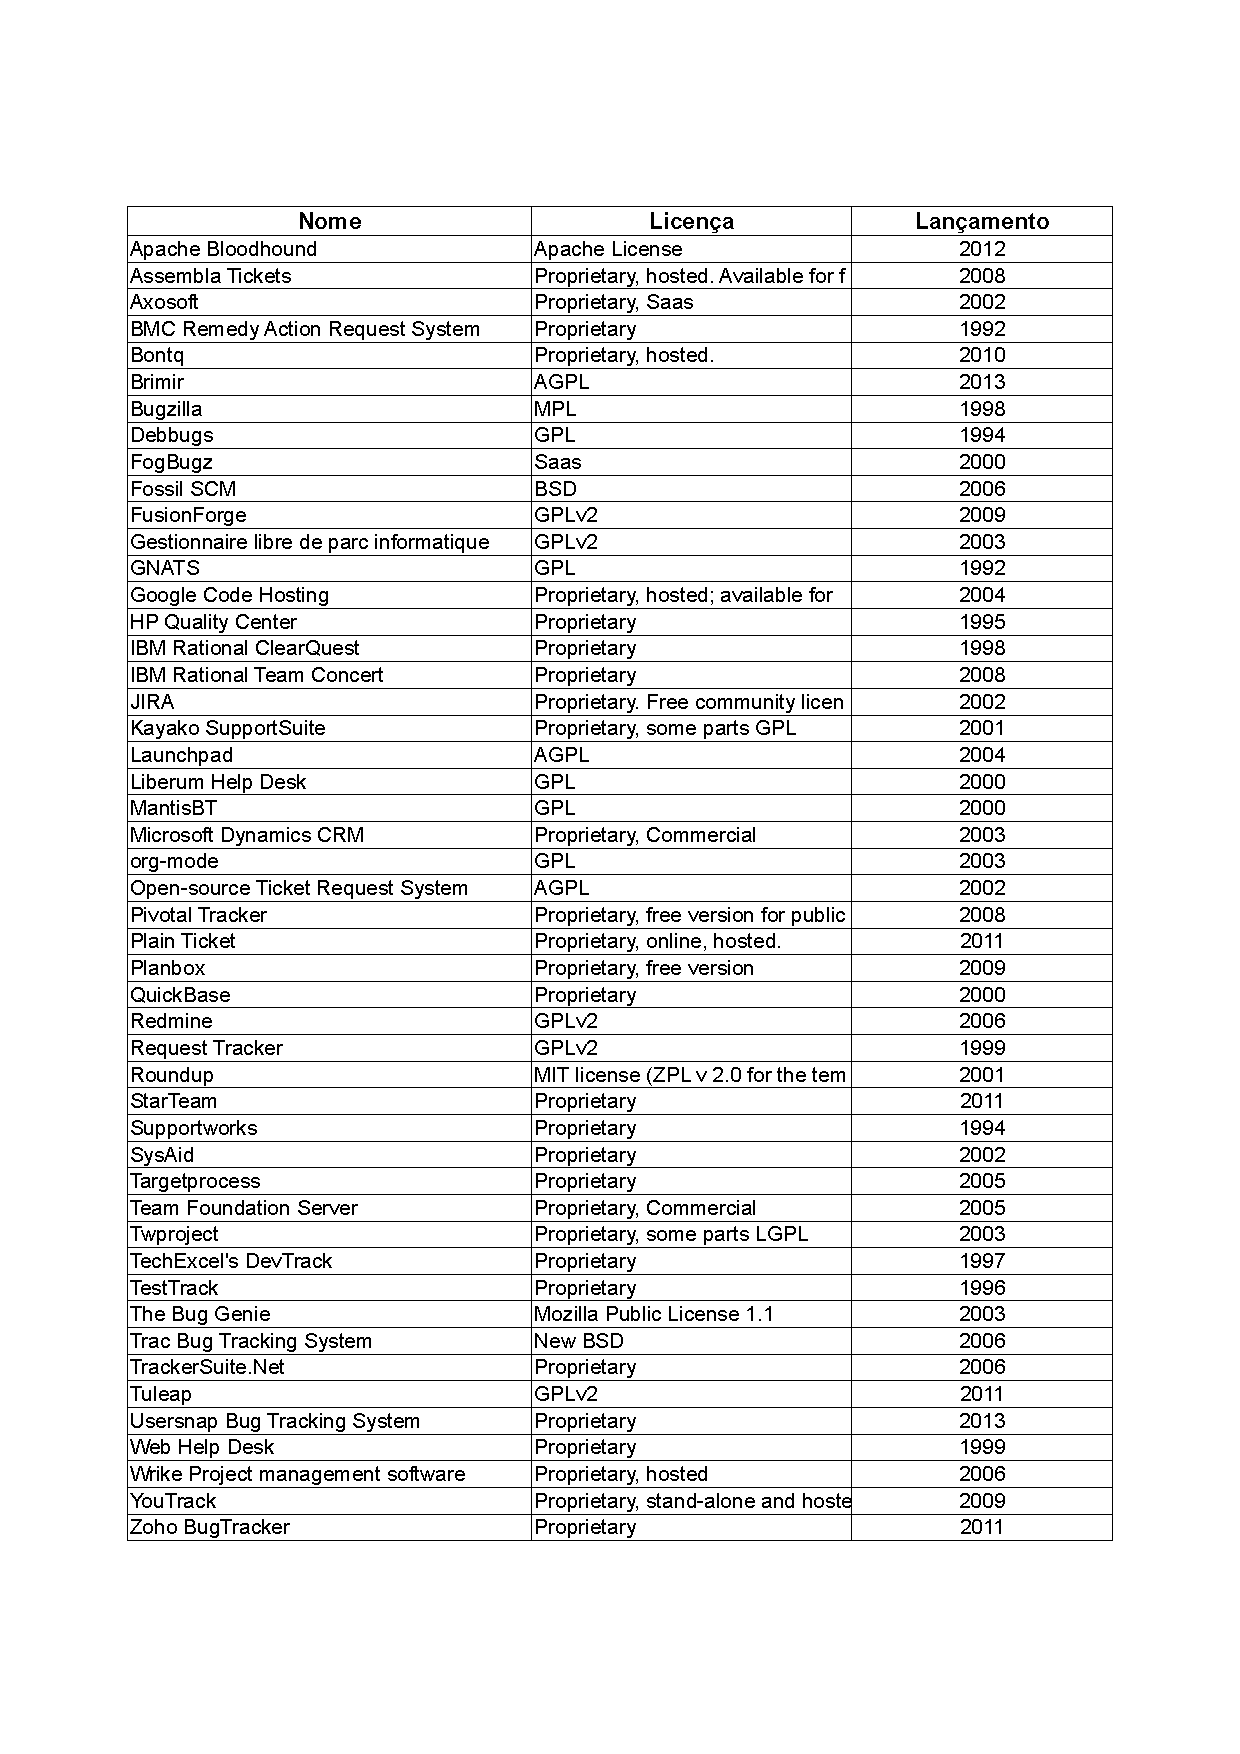
\includepdf[pages=-,scale=.8,linktodoc=true]{./apendices/img/Lista_ITS_Wikipedia.pdf}

\chapter{Formulário Aplicado para Seleção das Ferramentas}\label{ch:app-form-selecao-ferramentas}
\includepdf[pages=-,scale=.8,linktodoc=true]{./apendices/img/form-avalicao-ferramentas-pt-br.pdf}

\chapter{Modelo da Mensagem Enviada no Levantamento para Seleção das
    Ferramentas}\label{ch:app-template-msg-sel-ferrramentas}
\includepdf[pages=-,scale=.8,linktodoc=true]{./apendices/img/template-mensagem-escolha-ferramentas.eps}

\chapter{Formulário dos Cartões Ordenados}\label{ch:app-form-cartoes-ordenados}
\includepdf[pages=-,scale=.8,linktodoc=true]{./apendices/img/form-cartoes-ordenados.pdf}

\chapter{Sentenças de Busca por Base de Dados}\label{ch:app-setenca-de-busca-base-dados}
\includepdf[pages=-,scale=.8,linktodoc=true]{./apendices/img/setenca-de-busca-por-base-dados.pdf}

\chapter{Formulário Aplicado na Pesquisa com Profissionais}\label{ch:app-form-pesq-profissionais}
\includepdf[pages=-,scale=.8,linktodoc=true]{./apendices/img/form-melhorias-funcionalidades.pdf}

\chapter{Lista de Projetos Avaliação Sugestões de Melhorias}\label{ch:app-tb-lista-projetos-sug-melhorias}
\includepdf[pages=-,scale=.8,linktodoc=true]{./apendices/img/tb-lista-projetos-avaliacao-sug-melhorias.pdf}

\chapter{Formulário Aplicado para Avaliação das Sugestões de Melhorias}\label{ch:app-form-sug-melhorias}
\includepdf[pages=-,scale=.8,linktodoc=true]{./apendices/img/form-sugestoes-melhorias.pdf}

\end{appendices}

\end{document}
